% **************************************************
% Document Class Definition
% **************************************************
\documentclass[%
    paper=A4,               % paper size --> A4 is default in Germany
    twoside=true,           % onesite or twoside printing
    openright,              % doublepage cleaning ends up right side
    parskip=half,           % spacing value / method for paragraphs
    chapterprefix=true,     % prefix for chapter marks
    11pt,                   % font size
    headings=normal,        % size of headings
    bibliography=totoc,     % include bib in toc
    listof=totoc,           % include listof entries in toc
    titlepage=on,           % own page for each title page
    captions=tableabove,    % display table captions above the float env
    chapterprefix=false,    % do not display a prefix for chapters
    appendixprefix=false,   % but display a prefix for appendix chapter
    draft=false,            % value for draft version
]{scrreprt}%

\usepackage{enumitem}       
%\usepackage{layouts}       % Just to print the layout of this document
                            %     Please, remove in your version!


% **************************************************
% Setup YOUR master's thesis document in this file !
% **************************************************
% !TEX root = my-tfm.tex

% **************************************************
% Files' Character Encoding
% **************************************************
%% Not necessary with luaLaTeX
% 
\PassOptionsToPackage{utf8}{inputenc}
\usepackage{inputenc}


% **************************************************
% Information and Commands for Reuse
% **************************************************
\newcommand{\thesisTitle}{Sistema de autenticación continua basado en el comportamiento mediante técnicas de streaming}
\newcommand{\thesisName}{Arturo Silvelo Pallín}
\newcommand{\thesisSubject}{Trabajo Fin de Máster}
\newcommand{\thesisDate}{Curso 2020/2021}

\newcommand{\thesisFirstSupervisor}{José Carlos Dafonte Vázquez}
\newcommand{\thesisSecondSupervisor}{Daniel Garabato Míguez}

\newcommand{\thesisUniversityStudies}{\protect{Máster Inter-Universitario en Ciberseguridad}}
\newcommand{\thesisUniversity}{Universidad de A Coruña}     % Replace with your university
\newcommand{\thesisUniversitySchool}{Facultad de Informática} % Replace with your school
\newcommand{\thesisUniversityCity}{A Coruña}  % Replace with your city
\newcommand{\thesisUniversityStreetAddress}{Campus de Elviña}
\newcommand{\thesisUniversityPostalCode}{15071}


% **************************************************
% Debug LaTeX Information
% **************************************************
%\listfiles

% **************************************************
% Load and Configure Packages
% **************************************************
%\usepackage[spanish]{babel} % babel system, adjust the language of the content

\usepackage{polyglossia}
\setdefaultlanguage{spanish}

\PassOptionsToPackage{% setup clean thesis style
    figuresep=colon,
    hangfigurecaption=false,
    hangsection=true,
    hangsubsection=true,
    sansserif=false,
    configurelistings=true,
    colorize=full,
    colortheme=bluemagenta,
    configurebiblatex=true,
    bibsys=biber,
    bibfile=bib-refs,
    bibstyle=numeric-comp, %numeric-comp, numeric-verb, alphabetic 
    bibsorting=nty,
}{munics}
\usepackage{munics}

\hypersetup{% setup the hyperref-package options
    pdftitle={\thesisTitle},    %   - title (PDF meta)
    pdfsubject={\thesisSubject},%   - subject (PDF meta)
    pdfauthor={\thesisName},    %   - author (PDF meta)
    plainpages=false,           %   -
    colorlinks=false,           %   - colorize links?
    pdfborder={0 0 0},          %   -
    breaklinks=true,            %   - allow line break inside links
    bookmarksnumbered=true,     %
    bookmarksopen=true          %
}

% **************************************************
% Other Packages
% **************************************************
%\usepackage{fontspec}
\usepackage{scrhack}
\usepackage{subcaption}
\usepackage[justification=centering]{caption}
\usepackage{multirow}
\usepackage{booktabs}
\usepackage{tablefootnote}
\usepackage{amsmath}
\usepackage{makecell}
\usepackage{tabularx}
\usepackage{xltabular}
\usepackage{ragged2e}
\usepackage[official]{eurosym}
\usepackage{amsmath}
\usepackage{longtable}
\usepackage[capitalize]{cleveref}
\usepackage{xcolor}

% **************************************************
% Caption Setup
% **************************************************
\captionsetup{belowskip=12pt,aboveskip=4pt}

% **************************************************
% Tabular X
% **************************************************
\newcolumntype{C}{>{\Centering\arraybackslash}X} % centered "X" column
\newcolumntype{S}{>{\hsize=.4\hsize}X} % Small column

% **************************************************
% Formulas
% **************************************************
\DeclareMathOperator{\atantwo}{atan_2}
\makeatletter
\DeclareRobustCommand{\atan}{%
    \operatorname{atan}%
    \@ifnextchar2{_}{}%
}
\makeatother


% **************************************************
% Custom Figure
% **************************************************
\newcommand{\cfig}[4][.9\linewidth]{
    \begin{figure}[hbtp!]
        \centering
        \includegraphics[width=#1, keepaspectratio]{#2}
        \caption{#3}
        \label{#4}
    \end{figure}
}


% **************************************************
% Document CONTENT
% **************************************************
\begin{document}

% uncomment the following command to fill up pages with
% whitespace instead of aligning the first and last lines
% of a page (see \raggedbottom vs. \flushbottom)
%\raggedbottom

% --------------------------
% rename document parts
% --------------------------

% > set short label names for floating environments figure and table
\renewcaptionname{spanish}{\figurename}{Fig.}
\renewcaptionname{spanish}{\tablename}{Tab.}
\renewcommand{\lstlistingname}{List.}% Listing -> List.

\crefname{table}{Tabla}{Tablas}
\crefname{section}{Sección}{Sección}


% > rename the title of the LOL, i.e. list of listings (default is "Listings")
\renewcommand*{\lstlistlistingname}{Listado de extractos de código}

% --------------------------
% Front matter
% --------------------------
\pagenumbering{roman}			% roman page numbing (invisible for empty page style)
\pagestyle{empty}				% no header or footers
% !TEX root = ../my-tfm.tex
% ------------------------------------  --> main title page
\begin{titlepage}
	\pdfbookmark[0]{\thesisTitle}{\thesisTitle}
	% Different margins for the title page
	\newgeometry{left=1cm,right=1cm,top=10cm,bottom=6cm}
	\fontfamily{raleway}\selectfont
	\centering
	\MUniCSCover
	%\newfontfamily\raleway[Ligatures=TeX]{Raleway-Regular}
	\vfill
	{\fontsize{26pt}{26pt}\selectfont\raleway\color{white}\bfseries{\thesisTitle} \\[10mm]}
	{\fontsize{20pt}{20pt}\raleway\color{white}\thesisName} \\[5mm]
	{\raleway\color{lightgray} Tutores: \thesisFirstSupervisor\ e \thesisSecondSupervisor}
	\vfill

	{\raleway\color{white}\thesisDate}
	\restoregeometry

	% We restore the original margins

\end{titlepage}


% ------------------------------------  --> lower title back for single page layout

\clearpage
\begin{textblock*}{16cm}(2cm,\dimexpr\paperheight-8cm\relax)
	\small
	\textbf{\thesisName} \\
	\textit{\thesisTitle} \\
	\thesisSubject. \thesisDate \\
	Tutores: \thesisFirstSupervisor\ e \thesisSecondSupervisor \\[1.5em]
	\textbf{\thesisUniversityStudies} \\
	\textit{\thesisUniversity} \\
	\thesisUniversitySchool \\
	\thesisUniversityStreetAddress \\
	\thesisUniversityPostalCode, \thesisUniversityCity
\end{textblock*}
		% INCLUDE: all titlepages
\cleardoublepage

\pagestyle{plain}				% display just page numbers
% **************************************************
% Abstract
% **************************************************
\pdfbookmark[0]{Abstract}{Abstract}
\addchap*{Abstract}
\label{sec:abstract}

Nowadays, authentication systems allow to verify the user's identities at a specific point in the system, usually at login, while leaving the user with the responsibility of logging off each time they stop using their computer. Because of this step, in multiuser and professional environments, users often leave their sessions open so that other users can access and perform unauthorized operations on their behalf. These actions can result in access to confidential data that could cause legal problems for both the organization and the legitimate user, that may result in financial penalties.

To avoid these problems, new authentication systems have been developed, such as fingerprint schemes, but this entails a cost in price due to the installation of a reader for each workstation. Additionally, operating systems can implement restriction policies that close inactive sessions and force users to change their passwords in short periods of time. However, such measures may disturb the user and lead to the use of weak passwords, causing a false sense of security.


For this purpose, an authentication system has been proposed in this project as a second factor mechanism, in which the user's identities are periodically verified according to their behavior during their sessions. Thus, data related to mouse movement is gathered in order to build unique user profiles by means of Artificial Intelligence techniques that were combined with streaming processing methods to achieve a real-time authentication process. As a result, a scalable system able of authenticating users in a transparent manner to them was successfully developed and deployed.



{\vspace{5mm}\textbf{\textit{Keywords ---}}
    Mouse dynamics,
    Behavioral biometrics,
    Security monitoring
}


% **************************************************
% Resumen
% **************************************************
\pdfbookmark[0]{Resumen}{Resumen}
\addchap*{Resumen}
\label{sec:resumen}

Los sistemas de autenticación actuales permiten verificar la identidad de los usuarios en un momento concreto del sistema, por lo general al inicio, lo que deja al usuario la responsabilidad de cerrar la sesión cada vez que abandone su ordenador. Debido a este paso, en entornos multiusuario y en el ámbito profesional los usuarios suelen dejar sus sesiones abiertas permitiendo que otros usuarios accedan y realicen operaciones en su sesión. Estas acciones pueden derivar en acceso a datos confidenciales que provocarían problemas legales tanto a la organización como al usuario legítimo, resultando en posibles sanciones económicas.

Para evitar estos problemas se han implementado nuevos sistemas de autenticación, como los esquemas basados en la huella dactilar, pero esto conlleva un coste en precio debido a la necesidad de instalar un lector por cada puesto de trabajo. Por otra parte, los sistemas operativos permiten configurar políticas de restricción que cierran sesiones inactivas y obligan a los usuarios a cambiar sus contraseñas en cortos periodos de tiempo. Sin embargo, estas medidas pueden provocar malestar en los usuarios y llevar al uso de contraseñas débiles, lo que acaba provocando una falsa sensación de seguridad.


Para este propósito, en este proyecto se ha planteado un sistema de autenticación como segundo factor, en el que se verifica la identidad del usuario periódicamente a partir de su comportamiento en el uso del dispositivo. Para ello, se recopilan los datos relativos al movimiento del ratón para la creación de perfiles de usuario únicos con técnicas de Inteligencia Artificial que combinado con procesamiento \textit{streaming} realice el proceso de autenticación en tiempo real.  De esta manera, se ha implementado y desplegado un sistema escalable capaz de autenticar a los usuarios de manera transparente para ellos.


{\vspace{5mm}\textbf{\textit{Palabras clave ---}}
Movimientos de ratón,
Biometría del comportamiento,
Monitorización de seguridad
}
		% INCLUDE: the abstracts (english and galician)
\cleardoublepage

\pdfbookmark[0]{Agradecimientos}{Agradecimientos}
\addchap*{Agradecimientos}
\label{sec:acknowledgement}
\vspace*{\fill}
\begin{flushright}
	\small
	A mis padres	
\end{flushright}
 % INCLUDE: acknowledgement
\cleardoublepage

\currentpdfbookmark{\contentsname}{toc}
\setcounter{tocdepth}{3}		% define depth of toc --> 3 
\tableofcontents				% display table of contents
\cleardoublepage
% --------------------------
% Body matter
% --------------------------
\pagenumbering{arabic}			% arabic page numbering
\setcounter{page}{1}			% set page counter
\pagestyle{scrheadings}			% header and footer style

%% Uncomment the following lines using the \part command
%% to add part sections

\chapter{Introducción}
\label{sec:intro}

En este capítulo se expondrá una visión generalizada del proyecto, abordando la idea original del mismo, cómo surge y qué objetivos se pretenden conseguir con la realización de este.

\section{Motivación}
\label{sec:intro:motivacion}

Desde los inicios de la informática, la ciberseguridad~\cite{8906, stallings2012computer} ha sido una de las áreas de estudio que mayor interés ha despertado y, hoy en día, ha adquirido una especial relevancia en la vida cotidiana de los usuarios en prácticamente cualquier ámbito~\cite{EurostatComputerEmployees, EurostatComputerIndivual}, debido a la enorme proliferación de diferentes tipos de dispositivos, tales como ordenadores personales, tabletas o teléfonos inteligentes (smartphones), así como el uso habitual de diferentes plataformas y aplicaciones informáticas, como pueden ser productos de ofimática tradicionales, redes sociales, aplicaciones bancarias o plataformas de salud en línea. Actualmente, la ciberseguridad ha tomado una especial relevancia debido al creciente aumento de ataques informáticos a diferentes infraestructuras y plataformas, llegando a generar una gran preocupación no solo para las empresas responsables de dichos servicios, sino también para el usuario final de tales herramientas.

La seguridad informática abarca una gran variedad de técnicas y métodos para tratar de dotar a los sistemas de información de una cierta protección ante posibles ataques, incluyendo los sistemas físicos, los sistemas software o servicios, así como también la información almacenada en ellos. Entre estos mecanismos, se encuentran los sistemas de autenticación, un componente esencial en cualquier modelo de seguridad que actúa como un primer elemento de defensa de los sistemas de información mediante la verificación de la identidad de los usuarios. De este modo, una vez comprobada la identidad los sistemas de control de acceso podrán otorgar los permisos pertinentes a un usuario legítimo o bien denegar el acceso al sistema a un usuario ilegítimo, registrando y notificando dicha incidencia a los administradores del sistema.

Para llevar a cabo el proceso de autenticación, se emplean dos fases: en primer lugar, el usuario debe proporcionar una identificación para que, en un segundo paso, el sistema pueda llevar a cabo una comprobación para determinar si existe una correspondencia entre dicha identificación y la identidad del usuario. Actualmente existen diferentes maneras de realizar este procedimiento, en función del factor que se utilice para completarlo~\cite{barkadehi2018authentication}:

\begin{itemize}
    \item El esquema de autenticación más habitual está basado en un factor de conocimiento por parte del usuario y consiste en el uso de una determinada información que, teóricamente, solo deberían conocer el usuario legítimo y el sistema de autenticación, como pueden ser el uso de pares usuario/contraseña o números de identificación personal (PIN).
    \item Otro de los esquemas ampliamente utilizados, especialmente para llevar a cabo el control de acceso a edificios o áreas, es el factor de posesión, donde el usuario presenta al sistema autenticador un objeto o token para llevar a cabo la verificación de identidad. El uso de documentos acreditativos de identidad como el DNI o incluso las tarjetas bancarias son claros ejemplos de este tipo de sistemas, así como también podrían serlo el uso de tarjetas inteligentes de propósito específico o incluso la utilización de dispositivos móviles.
    \item Durante los últimos años también se han convertido en sistemas de autenticación habituales aquellos basados en factores biométricos, es decir, los que emplean ciertas propiedades inherentes a los usuarios que, además, son invariables en el tiempo para llevar a cabo la comprobación de la identidad, tales como la huella dactilar, el iris o incluso sistemas de reconocimiento facial~\cite{samangouei2017facial}.
    \item Uno de los sistemas más novedosos que está tomando cada vez una mayor relevancia se basa en realizar el proceso de autenticación apoyándose en la ubicación del usuario, empleando desde las direcciones MAC e IP del equipo utilizado, hasta el posicionamiento GPS a partir de la geolocalización de un dispositivo móvil~\cite{zhang2012location}.
    \item Otro tipo de sistemas que está tomando cada vez una mayor relevancia son los basados en factores de comportamiento biométrico~\cite{ahmed2005anomaly}, donde la verificación de la identidad de los usuarios se lleva a cabo a través de la monitorización de la interacción entre el propio usuario y el sistema, como por ejemplo el tipo de aplicación utilizada, los sitios Web frecuentados, la manera de teclear o incluso la utilización del ratón~\cite{bhatnagar2013survey,gamboa2003}.
\end{itemize}

A lo largo de los últimos años, los sistemas de autenticación han buscado reforzar el proceso añadiendo pasos complementarios en el proceso, requiriendo la presencia de múltiples factores para autenticar al usuario. Un claro ejemplo de este tipo de procedimientos son los sistemas de verificación en dos pasos [12], ampliamente extendidos hoy en día, donde se lleva a cabo una autenticación mediante un factor primario, habitualmente basado en un esquema usuario/contraseña, solicitando posteriormente al usuario un código de confirmación enviado a su dispositivo móvil, bien sea un SMS o a través de una aplicación específica.

Mediante la utilización de los métodos anteriormente señalados, es importante resaltar que la identidad del usuario solamente se verifica en el momento inicial y, por tanto, podría darse una usurpación de una sesión abierta. Ante este tipo de circunstancias, empleando mecanismos de autenticación convencionales únicamente sería posible prevenir este tipo de situaciones mediante la repetición periódica de todo el proceso de autenticación, lo que dificultaría la experiencia del usuario al tratarse generalmente de procesos invasivos que interrumpirían la sesión. Por tanto, para llevar a cabo este proceso de forma transparente al usuario será necesario recurrir a factores de autenticación no invasivos, un perfil en el que encajan perfectamente los factores basados en el comportamiento del usuario. De este modo, sería posible monitorizar la actividad del usuario de forma constante, completando el proceso de autenticación de forma continuada y permitiendo la detección de posibles suplantaciones de identidad [13].

El trabajo que se ha realizado en este proyecto se centra precisamente en estos sistemas de autenticación de segunda fase basados en el comportamiento del usuario frente al dispositivo que emplea, en este caso orientado a explotar la interacción mediante un dispositivo convencional, como es el ratón. Para ello, el usuario debe completar el proceso de autenticación inicial para la apertura de sesión mediante un factor primario (usuario/contraseña) y, posteriormente, la verificación continua de su identidad se llevará a cabo de forma recurrente y totalmente transparente para el usuario.

Aquí nos planteamos un sistema de monitorización en tiempo real y sobre entornos de trabajo reales. De esta forma, las capturas asociadas al comportamiento se realizarán en un entorno no controlado, es decir, entornos en los que el usuario tendrá libertad de movimientos y no será un escenario guiado. Estas nos proporcionarán eventos que posteriormente convertiremos en características. Aplicando sobre estas características diferentes técnicas de Inteligencia Artificial, podremos encontrar patrones que permitan autenticar al usuario. Todos los datos del sistema se procesarán mediante una plataforma de \textit{streaming} de datos, que permitirá realizar el proceso de autenticación en tiempo real. 


\section{Objetivos}
\label{sec:intro:objetivos}

El proyecto debe cumplir los siguientes objetivos, para garantizar la calidad y funcionalidad del mismo:

\begin{enumerate}[noitemsep]
    
    \item Implementar una aplicación de escritorio que permita la captura de los eventos del usuario para su posterior envío. El lenguaje de programación elegido deberá permitir generar un aplicativo multiplataforma.
    
    \item Implementar un servidor que permita la distribución de los mensajes. Estudiando las propuestas y estándares disponibles y  seleccionando una plataforma de distribución de mensajes que permita un gran volumen de tráfico. Además, la opción elegida deberá contar con la opción de incrementar sus funcionalidades base mediante \textit{plugins} o librerías.
    
    \item Realizar una fase de recogida de información con la aplicación de escritorio creada, con el fin de obtener un conjunto de datos que contenga una muestra representativa de la población, es decir, personas de diferentes edades y géneros.
    
    \item Analizar la información recopilada, planteando, desarrollando y evaluando diferentes mecanismos de autenticación basados en el estudio de patrones de comportamiento de los usuarios mediante múltiples técnicas de Inteligencia Artificial, como pueden ser redes neuronales~\cite{werbos2008foreword}, máquinas de soporte vectorial~\cite{cortes1995support} o árboles aleatorios~\cite{Breiman2001}. Por otro lado, también será necesario estudiar las diferentes características del comportamiento de los usuarios y determinar aquellas de mayor relevancia para acometer el proceso de autenticación, generando perfiles únicos por usuario.
    
    \item Implementar un servicio que permita la automatización del proceso de creación de modelos únicos para cada usuario.
    
    \item Implementar una aplicación web que permita visualizar los datos generados y el estado del 
    sistema de una manera sencilla. Este desarrollo se debe realizar con un \textit{framework} que agilice su programación y mantenimiento.  

\end{enumerate}

\section{Organización de la memoria}
\label{sec:intro:organizacion}

La memoria se estructura basándose en una serie de capítulos:

\begin{itemize}[noitemsep]
    \item \textbf{Fundamentos teóricos:} En este capítulo se abordan los diferentes términos para comprender mejor el dominio.
    \item \textbf{Situación actual:} En este capítulo se muestra algunas de las alternativas disponibles y artículos encontrados relacionados con el tema que se trata en el proyecto.
    \item \textbf{Planificación y evaluación de costes:} En este capítulo se exponen las fases del desarrollo del proyecto, su realización, costes, recursos y riesgos asociados.
    \item \textbf{Tecnologías:} En este capítulo se analizan las herramientas utilizadas para el desarrollo del proyecto y las decisiones tomadas para su elección.
    \item \textbf{Metodología:} En este capítulo se muestra la información relativa al desarrollo del proyecto.
    \item \textbf{Inteligencia Artificial:} En este capítulo se muestra el procedimiento realizado para el proceso de creación de los modelos de los usuarios.
    \item \textbf{Kafka - Sistemas de colas:} En este capítulo se muestra el proceso de implementación y creación del sistema de gestión de colas.
    \item \textbf{Resultados:} En este capítulo se exponen y discuten los resultados obtenidos.
    \item \textbf{Conclusiones:} En el último capítulo de la memoria se comprobará el grado de cumplimiento de los requisitos y su impacto. 
    \item \textbf{Trabajo Futuro:} En este capítulo se expondrá las diferentes ramas de desarrollo que se han tenido en cuenta para la continuación del proyecto.
 
\end{itemize}

\chapter{Fundamentos teóricos}
\label{sec:fundamentos}


En este capítulo se presentarán las principales temáticas relacionadas con el dominio del proyecto, con el objetivo de comprenderlo mejor.

\section{Seguridad Informática}
La seguridad informática forma parte de un término más genérico como es la seguridad de la información, y tiene como objetivo prevenir y detectar el uso no autorizado de un sistema informático.

\subsection{Conceptos previos}

\begin{itemize}
    \item \textbf{Atacante:} Sujeto o entidad que pone en riesgo un sistema.

    \item \textbf{Ataque}: Consiste en cualquier acción hecha por individuos u organizaciones  que roban, alteran o destruyen a un blanco específico.
          \begin{itemize}
              \item \textbf{Ataque pasivo:} Son ataques difíciles de detectar, puesto que el atacante solo observa o monitoriza la información.

              \item \textbf{Ataque activo:} Son aquellos que implican algún tipo de modificación de la información con el fin de dañar al objetivo.

          \end{itemize}

    \item \textbf{Intrusión:} Conjunto de acciones que intentan comprometer la integridad, confidencialidad o disponibilidad de un recurso. Es decir, la intrusión no solo consiste en el acceso no autorizado, sino también en la denegación del acceso a otros usuarios o la manipulación de la información.

    \item \textbf{Vulnerabilidad~\cite{incibe_2017}:} Debilidad o fallo en un sistema de información que pone en riesgo la seguridad de la información, permitiendo que un atacante pueda comprometer la integridad, disponibilidad o confidencialidad de la misma.


    \item \textbf{Amenaza~\cite{incibe_2017}:} Acción que aprovecha una vulnerabilidad para atentar contra la seguridad de un sistema de información. Es decir, que podría tener un potencial efecto negativo sobre algún elemento de nuestro sistema.

    \item \textbf{Riesgo~\cite{incibe_2017}:} El riesgo es la probabilidad de que se produzca un incidente de seguridad, materializándose una amenaza y causando pérdidas o daños.

    \item \textbf{Política de Seguridad~\cite{rediris_2002_security}}: Conjunto de requisitos definidos por los responsables de un sistema que indican en términos generales qué está y qué no está permitido en el área de la seguridad durante el uso del sistema.

\end{itemize}



\subsection{Objetivos de la seguridad informática}
Los sistemas de información guardan, distribuyen o generan información para usuarios, empresas, procesos o aplicaciones, y esta información debe garantizar ciertas características para evitar fraudes. La seguridad informática intenta asegurar estas garantías sobre la información~\cite{rediris_2002_introduction}:

\begin{itemize}
    \item \textbf{Confidencialidad}: Es la capacidad de que solo los usuarios autorizados puedan acceder a nuestros recursos, datos e información. Este es uno de los principales problemas a los que se enfrentan las empresas.
    \item \textbf{Integridad}: Es la capacidad de asegurar que los datos sean legítimos, es decir, asegurar que los datos recibidos sean los generados inicialmente y que nada, ni nadie ajeno pueda modificar dichos datos.
    \item \textbf{Disponibilidad}: Esta característica es de las más importantes y asegura que los datos estén accesibles siempre que el usuario, proceso o sistema lo necesite.


\end{itemize}


\subsection{Autenticación de usuario}
En el ámbito de la seguridad informática es muy importante demostrar que un usuario o una aplicación es realmente quien dicha persona o aplicación asegura ser. Para esta verificación se pueden usar varias técnicas~\cite{rediris_2002_auth}:

\begin{enumerate}
    \item \textbf{Sistemas basados en algo conocido}: Es el modelo de autenticación más básico y consiste en decidir si un usuario dice ser quien es simplemente basándonos en una prueba que a priori solo ese usuario puede saber. Esta aproximación es la más barata y también la más vulnerable a todo tipo de ataques. Las entidades que participan en la autenticación acuerdan una clave, que mantendrán en secreto. Cuando una de las partes necesita autenticarse solo tiene que mostrar la clave secreta que han acordado para poder acceder a los recursos.

    \item \textbf{Sistemas basados en algo poseído}: Este modelo de autenticación es más complejo y se puede complementar con otros sistemas como el anterior de una manera fácil, pero también implica un mayor coste. Por lo general, este modelo se caracteriza por el uso de una tarjeta con un chip integrado el cual incorpora la información necesaria para la autenticación del usuario.
          Este dispositivo fue patentado por \textbf{Roland Moreno} en 1970, y consistía en una tarjeta de plástico con un chip integrado. A día de hoy este tipo de tarjeta está presente en multitud de aplicaciones como tarjeta bancarias, tarjetas de acceso, etc.
    \item \textbf{Sistemas de autenticación biométrica}: Hoy en día existen otros mecanismos que se basan en las cualidades del usuario.
          Este tipo de sistemas basados en el reconocimiento de cualidades físicas del usuario, utilizan características únicas del individuo para su identificación. El proceso general para este tipo de sistemas es el siguiente:
          \begin{enumerate}[label={\arabic*.}]
              \item Capturar una muestra de los datos del usuario.
              \item Extraer las características que sean únicas de ese usuario.
              \item Comparar dichas características con las extraídas en un primer momento.
              \item Basándonos en esa comparación se decide si el usuario es quien dice ser.
          \end{enumerate}

          Los sistemas de autenticación biométricos más comunes son:
          \begin{itemize}
              \item \textbf{Verificación de huella dactilar}: La huella de un ser humano es un rasgo de identificación único (salvo alguna excepción), pero los sistemas de autenticación miden ciertas características que se han demostrado únicas en los todos los individuos~\cite{mseg}.

              \item \textbf{Verificación de patrones oculares}: Estos modelos de reconocimiento mediante patrones oculares, por lo general miden rasgos en el iris o en la retina. Han demostrado ser los más fiables con una probabilidad de coincidencia cercana a cero.

          \end{itemize}

          Otros sistemas de autenticación biométricos basados en el comportamiento humano, como el que se trata en este proyecto, son:

          \begin{itemize}
              \item \textbf{Reconocimiento de voz}: El reconocimiento de voz intenta detectar características típicas de la voz del usuario para identificarlo. La técnica aplicada para lograr este fin es similar a los sistemas de reconocimiento de canciones como \textit{shazam}~\cite{WangAvery}.


              \item \textbf{Verificación de escritura}: Estos sistemas intentan verificar la firma manuscrita de una persona. En ella se verifican los patrones y características del trazo realizado.

                    %   \item \textbf{Sistemas de reconocimiento de escritura por teclado}~\cite{daniel_garabato}: Este tipo de sistemas intenta caracterizar al usuario a partir de ciertos patrones que se producen cuando escribe con un teclado.

                    %   \item \textbf{Sistemas de reconocimiento mediante el uso del ratón}~\cite{jorge_rodriguez}: Intentan caracterizar a los usuarios mediante el estudio de las curvas que se trazan cuando se realizan movimientos con el ratón

          \end{itemize}



\end{enumerate}



\section{Características del uso del ratón}

Los datos en bruto generados por un ratón~[\cref{tab:raw_inputs}] deben ser procesados para extraer aquellas características relevantes para el problema y que pueden ser tratadas adecuadamente por las técnicas de aprendizaje automático.

Para este propósito se analizaron diferentes propuestas de la literatura que utilizan características de distinta naturaleza, principalmente basadas en propiedades del movimiento~\cite{sayed2013,zheng2011,gamboa2003} como velocidades, aceleraciones y variaciones de ángulo. En este proyecto, nos hemos centrado en las características basadas en el movimiento, ya que el objetivo es obtener un sistema de autenticación basado en el comportamiento. En consecuencia, hemos seleccionado como referencia las características de~\cite{gamboa2003} y  hemos incluido nuevas características que se derivan de estas aplicando las siguientes técnicas:
\begin{itemize}
    \item Valores absolutos: Obtenidos a partir de las características originales.
    \item Descomposición en características básicas: Algunas características se descomponen en valores más primitivos, como la velocidad que se divide en horizontal y vertical.
    \item Hemos decidido agrupar los eventos, tomando el primer evento como origen y calculando las características respecto a él.
\end{itemize}

La totalidad de las características extraídas son detalladas en la~\cref{tab:transform_inputs}.


\begin{table}[htbp!]
    \centering
    \begin{tabular}{ c  l }
        \toprule
        \textbf{Característica} & \textbf{Definición}                                    \\
        \midrule \midrule
        x                       & Posición del ratón en el eje horizontal de la pantalla \\
        
        y                       & Posición del ratón en el eje vertical de la pantalla   \\
        
        \textit{timestamp}               & Instante de tiempo del movimiento (formato UNIX)       \\
        \bottomrule
    \end{tabular}
    \caption{\label{tab:raw_inputs}Valores de entrada de un movimiento}
\end{table}




\begin{xltabular}[c]{\linewidth}{ l c }
    \toprule
    \textbf{Característica} & \textbf{Definición}\\
    \midrule \midrule
    \textit{Horizontal Velocity} &  $ hv =  \frac{x_i - x_j}{t_i - t_j}$ \\ \midrule
    \textit{Absolute Horizontal Velocity} & $ hv\_abs = |hv|$ \\ \midrule
    \textit{Horizontal Velocity Left} &
    $ hv_l =
        \begin{cases}
            hv\_abs, & \text{if}\ hv > 0 \\
            0,       & \text{otherwise}
        \end{cases}
    $ \\ \midrule
    \textit{Horizontal Velocity Right} &
    $ hv_r =
        \begin{cases}
            hv\_abs, & \text{if}\ hv < 0 \\
            0,       & \text{otherwise}
        \end{cases}
    $ \\ \midrule
    \textit{Vertical Velocity} &  $ vv = \frac{x_i - x_j}{t_i - t_j}$\\ \midrule
    \textit{Absolute Vertical Velocity} & $ vv\_abs = |vv|$ \\ \midrule
    \textit{Vertical Velocity Left} &
    $ vv_l =
        \begin{cases}
            vv\_abs, & \text{if}\ vv > 0 \\
            0,       & \text{otherwise}
        \end{cases}
    $ \\ \midrule
    \textit{Vertical Velocity Right} &
    $ vv_l =
        \begin{cases}
            vv\_abs, & \text{if}\ vv < 0 \\
            0,       & \text{otherwise}
        \end{cases}
    $ \\ \midrule
    \textit{Tangencial Velocity} & $ tv = \sqrt{hv^2 + vv^2}$ \\ \midrule
    \textit{Tangencial Acceleration} & $ ta = \frac{tv_i - tv_j}{t_i - t_j} $ \\ \midrule
    \textit{Absolute Tangencial Acceleration} & $ ta\_abs = |ta| $ \\ \midrule
    \textit{Tangencial Jerk} & $ tj = \frac{ta_i - ta_j}{t_i - t_j} $ \\ \midrule
    \textit{Absolute Tangencial Jerk} & $ tj\_abs = |tj| $ \\ \midrule
    \textit{Tangencial Jerk Left} &
    $ tj_l =
        \begin{cases}
            tj\_abs, & \text{if}\ tj > 0 \\
            0,       & \text{otherwise}
        \end{cases}
    $ \\ \midrule
    \textit{Tangencial Jerk Right} &
    $ tj_r =
        \begin{cases}
            tj\_abs, & \text{if}\ tj < 0 \\
            0,       & \text{otherwise}
        \end{cases}
    $ \\ \midrule
    \textit{Origin Distance} & $ d_o = \sqrt{x^2 + y^2}$  \\ \midrule
    \textit{Distance} & $ d = \sqrt{(x_i - x_y)^2 + (y_i - y_j)^2} $ \\ \midrule
    \textit{Slope Angle Tangent} & $ts\_angle = \atan2(y,x)$ \\ \midrule
    \textit{Origin Slope Angle Tangent} & $ts\_{origin\_angle} = \atan2(y_i - y_o, x_i -x_o)$ \\ \midrule
    \textit{Curvature} & $c = \frac{ts\_angle_i - ts\_angle_j}{t_i - t_j} $ \\ \midrule
    \textit{Absolute Curvature} & $c\_abs = |c| $ \\ \midrule
    \textit{Curvature Rate} &  $cr = \frac{c_i - c_j}{d_j - d_i}$ \\ \midrule
    \textit{Absolute Curvature Rate} &  $ cr\_abs = |cr|$ \\ \midrule
    \textit{Origin Curvature} &
    $ c\_origin =
        \frac{ts\_origin\_angle_o - ts\_origin\_angle_j}
        {t_o - t_j}$ \\ \midrule
    \textit{Absolute Origin Curvature} &  $ c\_origin\_abs = |c\_origin|$ \\ \midrule
    \textit{Origin Curvature Rate} &  $ cr\_origin = \frac{c_o - c_j}{t_o - t_j}$ \\ \midrule
    \textit{Absolute Origin Curvature Rate} & $ cr\_origin\_abs = |cr\_origin| $ \\ \midrule
    \multicolumn{2}{p{11cm}}{\footnotesize donde $x$ es la posición del ratón, $t$ es el \textit{timestamp} del evento, $o$ es el registro origen, $i$ es el registro actual y $j$ el registro anterior.} \\
    \bottomrule
    \caption{\label{tab:transform_inputs}Lista de características transformadas}
\end{xltabular}


\section{Evaluación del rendimiento}
\label{sec:metrics}

Para analizar los resultados obtenidos y comprobar la fiabilidad de los algoritmos usados, necesitamos emplear unas métricas que evalúen su rendimiento y permitan comparar diferentes aproximaciones.


El conjunto de datos utilizados para la evaluación del rendimiento consistirá en un \textit{dataset} con los datos distribuidos en dos grupos, los datos del usuario legítimo, que son los eventos obtenidos de la sesión de ese usuario, frente a los datos del usuario ilegítimo, que son los eventos capturados de otros usuarios. La distribución de este conjunto se realizará en una proporción 1:1.

Para evaluar el rendimiento de los algoritmos se empleará la matriz de confusión~[\cref{fig:matrix_conf}], la cual categoriza los datos en cuatro grupos:    


\begin{itemize}
    \item \textbf{Verdaderos Negativos (TN)}: Es la cantidad de eventos de usuarios no legítimos que fueron clasificados correctamente.

    \item \textbf{Falsos Positivos (FP)}: Es la cantidad de eventos de usuarios no legítimos que fueron clasificados incorrectamente como legítimos.

    \item \textbf{Falsos Negativos (FN)}: Es la cantidad de eventos del usuario legítimo que fueron clasificados incorrectamente como no legítimos.

    \item \textbf{Verdaderos Positivos (TP)}: Es la cantidad de eventos del usuario legítimo que fueron clasificados correctamente.
\end{itemize}


\cfig[0.6\linewidth]{images/fundamentos/matriz_confusion.png}{Esquema matriz de confusión.}{fig:matrix_conf}

A partir de los datos obtenidos de una matriz de confusión, se pueden calcular medidas que permiten obtener una representación analítica de los resultados. Por otra parte, durante el entrenamiento de los algoritmos también se han calculado los tiempos de cómputo.

\begin{itemize}
    \label{list:scores}
    \item\textbf{Recall (RC)}: Es la relación entre las predicciones positivas correctas y el total de observaciones positivas.
    \begin{equation}
        \frac{TP}{TP + FN}
    \end{equation}

    \item \textbf{Precision (PS)}: Es la relación entre las predicciones positivas correctas y el total de predicciones positivas.
          \begin{equation}
              \frac{TP}{TP  + FP}
          \end{equation}

    \item \textbf{F1}: Es la media armónica de los valores anteriores.
          \begin{equation}
              \frac{2}{\frac{1}{precision} + \frac{1}{recall}} = 2 * \frac{precision *
                  recall}{precision + recall} = \frac{TP}{TP + \frac{FN + FP}{2}}
          \end{equation}

    \item \textbf{Accuracy}: Es la relación entre las predicciones positivas y el total de casos.
          \begin{equation}
              \frac{TP}{TP + FP + FN + TN}
          \end{equation}
\end{itemize}

A partir de los datos de la matriz de confusión y un umbral (\textit{threshold}) es posible calcular ciertos ratios que permiten parametrizar de una manera más objetiva el rendimiento del algoritmo. Estos ratios son los definidos a continuación:

\begin{itemize}
          \item \textbf{Threshold:} Es un valor que se elige para considerar si el modelo de predicción es correcto o no. Este valor indica el grado de sensibilidad para rechazar casos falsos positivos y casos de falsos negativos.

          \item \textbf{False Acceptance Rate (FAR)~[\cref{fig:frr_far_chart}]:} Representa el ratio de casos en el que un usuario no legítimo es clasificado como legítimo. En el \textit{threshold} 0, la probabilidad de esta identificación es del 100\% e irá disminuyendo cuando se baja el \textit{threshold}.
          \begin{equation}
              \frac{FP}{FP+TN}
          \end{equation}

          \item \textbf{False Reject Rate (FRR)~[\cref{fig:frr_far_chart}]:} Representa el ratio de casos en el que un usuario legítimo es clasificado como no legítimo. En el \textit{threshold} 0, el usuario legítimo será identificado correctamente el 100\% de los casos e irá disminuyendo cuando se baja el \textit{threshold}.
          \begin{equation}
              \frac{FN}{FN+TP}
          \end{equation}
          
          \item \textbf{Equal Error Rate (EER)~[\cref{fig:frr_far_chart}]:} Representa el punto óptimo de \textit{threshold} donde las curvas de \textit{FRR} y \textit{FAR} se cortan, este valor suele ser mejor cuanto más cercano a cero se encuentre.
              \begin{equation}
                  \frac{FAR + FRR}{2}
              \end{equation}

\end{itemize}

\cfig{images/fundamentos/FAR-FRR-EER-Biometrics-schema.png}{Relación de EER con FAR y FRR}{fig:frr_far_chart}

\section{Inteligencia Artificial}

En 1956, \textbf{John McCarthy}~\cite{mccarthy2007artificial}, conocido como el padre de la Inteligencia Artificial, acuñó el término Inteligencia Artificial, en adelante \textit{IA}, como la ciencia y la ingeniería de hacer máquinas inteligentes, especialmente programas informáticos inteligentes.

En la \textit{IA} existen dos grupos definidos, fuerte y débil. La  \textit{IA} fuerte es aquella que tiene las mismas características que un humano inteligente. La \textit{IA} débil es aquella que muestra inteligencia en un área en concreto, pero carece de la misma en otras.

Para conseguir dotar de inteligencia a una máquina se suele utilizar el aprendizaje máquina o \textit{machine learning}. El aprendizaje máquina, en adelante \textit{ML}, es una de las áreas más extendidas de la \textit{IA}. En 1959, \textbf{Arthur Samuel} definió \textit{ML} como el campo de estudio que brinda a las computadoras la capacidad de aprender sin estar programado explícitamente.

\subsection{Tipo de aprendizaje}

Dentro del \textit{ML} se pueden distinguir dos tipos de aprendizaje:

\begin{itemize}
    \item \textbf{Aprendizaje supervisado}: Los algoritmos son entrenados basándose en un conjunto de datos de los que conocemos su respuesta correcta. De esta manera lo que se intenta es que el algoritmo obtenga una respuesta aceptable a partir de las características disponibles.

          \begin{itemize}
              \item \textbf{Problemas de regresión}: Son usados para evaluar las relaciones que existen entre las variables y obtener un valor de esa estimación.
              \item \textbf{Problemas de clasificación}: Son utilizados para dividir un conjunto de datos de entrada en distintas clases según sus características.
          \end{itemize}

    \item \textbf{Aprendizaje no supervisado}: En este modelo, los datos no contienen una respuesta correcta. Este tipo de aprendizaje intenta buscar ciertos patrones para obtener una respuesta aceptable.
\end{itemize}

La finalidad de todos estos tipos de aprendizajes es la de generalizar, es decir, que puedan resolver problemas que no han visto previamente.
Cuando entrenamos modelos computacionales con un conjunto de datos de entrada estamos haciendo que el algoritmo sea capaz de generalizar un concepto para que al consultarle por un nuevo conjunto de datos desconocido, este sea capaz de comprenderlo y proporcionarnos un resultado fiable~[\cref{fig:over-under-fitting}].

Si nuestros datos de entrenamiento son muy pocos o poco representativos nuestra máquina no será capaz de generalizar el conocimiento y estará incurriendo en \textit{underfitting}~[\cref{fig:over-under-fitting}].

Si sobreentrenamos (\textit{overfitting}) nuestro modelo lo que ocurrirá es que nuestra máquina solo se limitará a memorizar los casos particulares que le enseñamos y será incapaz de reconocer nuevos datos de entrada, perdiendo toda capacidad de generalización.

\cfig{images/fundamentos/overfitting.png}{Problemas de entrenamiento}{fig:over-under-fitting}


\subsection{Redes Neuronales Artificiales}
Las redes neuronales artificiales~\cite{salas2004redes}, en adelante \textit{RNA}, son un modelo computacional inspirado en la estructura del sistema nervioso de los seres humanos. La unidad elemental de una \textit{RNA} es la neurona artificial [\cref{fig:neurona}] y generalmente están organizadas en capas. Poseen una capa de entrada con \textit{n} entradas y una capa de salida con \textit{m} salidas, que se calcula normalmente realizando una suma ponderada de las entradas con sus pesos~[\cref{eq:perceptron}].


\begin{equation} \label{eq:perceptron}
    \displaystyle\sum_{i=1}^{n} w_i x_i + w_0=
    \begin{cases}
        \geq 0 & \quad y = 1 \\
        <    0 & \quad y = 0
    \end{cases}
\end{equation}

, donde $x_i$ son las entradas, $w_i$ es el peso de cada entrada y $w_0$ es el valor de \textit{bias}.



Este resultado es modificado por una función de activación y el valor obtenido se transmite directamente al siguiente elemento. Normalmente para conseguir esta transformación se emplean las funciones comentadas en la~\cref{tab:functions_mlp}.

\begin{table}[htbp!]
    \centering
    \begin{tabular}{l c}
        \toprule
        \textbf{Función} & \textbf{Ecuación}\\ \midrule
        Sigmoidal       &  $f(x) = \frac{1}{1 + e^{-x}}$ \\ \midrule
        Tangente hiperbólica       & $f(x) = tanh(x)$ \\ \midrule
        Gaussiana       & $ f(x) = e^{\frac{-x^2}{2}}$  \\ 
        \bottomrule
    \end{tabular}
    \caption{Funciones de activación}
    \label{tab:functions_mlp}
\end{table}


\cfig{images/fundamentos/neurona.jpg}{Esquema de una neurona artificial}{fig:neurona}

\subsubsection{Perceptrón Multicapa}
\label{sec:mlp}

En 1958, \textbf{Rosenblatt}~\cite{rosenblatt1960perceptron} diseñó y desarrollo el perceptrón. Este modelo implementa el funcionamiento de una sola neurona que es capaz de resolver problemas lineales. En 1969, \textbf{Minsky y Papert} escribieron un libro~\cite{minsky2017perceptrons} donde demostraron que un solo perceptrón era incapaz de aprender la función exclusiva (XOR), es decir, problemas cuya resolución no es lineal. En este mismo libro se expone un nuevo paradigma de \textit{RNA} llamado perceptrón multicapa  también conocido como \textit{MLP} por sus siglas en inglés (\textit{Multi-Layer Perceptron}). Este modelo es una combinación de varios perceptrón, que permiten aproximar cualquier problema, aunque no sea lineal. Este se caracteriza por tener sus neuronas agrupadas en capas de diferentes niveles, por lo general tres~[\cref{fig:schematic_MLP}].

\begin{itemize}
    \item \textbf{Capa de entrada:} Esta capa conecta la red con el exterior, cada neurona se corresponde con cada una de las variables de entrada a la red.

    \item \textbf{Capas ocultas:} Es un conjunto de capas que cuyas entradas son las salidas de la capa anterior y cuya salida pasan a la capa sucesora.

    \item \textbf{Capa de salida:} Conecta las capas ocultas con la salida de la red que proporciona los resultados.
\end{itemize}

Además, sus conexiones están dirigidas hacia adelante, es decir, las neuronas de una capa se conectan con las neuronas de la siguiente capa y generalmente todas las neuronas de una capa se encuentran enlazadas con las de la siguiente capa.

\cfig{images/fundamentos/schematic_mlp.png}{Esquema del MLP}{fig:schematic_MLP}


Inicialmente, este planteamiento no se pudo materializar porque no existía un mecanismo que ajustase automáticamente los pesos de la capa oculta. En 1986, \textbf{Rummelhart, Hinton y Wiliams} desarrollan la \textit{Regla Delta Generalizada}~\cite{rumelhart1988learning} para adaptar los pesos propagando los errores hacia atrás. De esta manera se demuestra que el \textit{MLP} es capaz de resolver problemas lineales y no lineales.

En la \cref{fig:MLP_example} se puede ver el funcionamiento del \textit{MLP}. En ella se muestra el esquema de un \textit{MLP} que contiene una capa de entrada, dos capas ocultas y la salida.
Cada neurona está representada visualmente con una gráfica que muestra la función aplicada a los datos, por ejemplo, en la capa de entrada, las variables de entrada son dos funciones que dividen los datos en vertical~($X_1$) y horizontal~($X_2$). También se pueden observar las distintas conexiones que existen entre las neuronas e incluso el peso de las conexiones representadas por un color y grosor diferentes.

\cfig{images/fundamentos/MLP_example.png}{Ejemplo de una MLP}{fig:MLP_example}

Este tipo de arquitectura es muy utilizada debido a su capacidad de aproximación universal. No obstante, necesitan un largo proceso de aprendizaje para problemas complejos que requieren de un gran número de variables y una arquitectura compleja.


% ======================================================== %

% ======================================================== %

\subsection[Máquinas de soporte vectorial]{Máquinas de soporte vectorial~\cite{berwick2003idiot}}
\label{sec:svm}
Las máquinas de soporte vectorial también conocidas como \textit{SVM} de sus siglas en inglés (\textit{Support Vector Machines}), es un conjunto de algoritmos desarrollados por \textbf{Vladimir Vapnik}, capaces de realizar clasificaciones, regresiones e incluso detectar valores atípicos.


Las \textit{SVM} generan un hiperplano\footnote{Es un plano de una dimensión inferior al origen, que divide el espacio en dos mitades} para intentar clasificar los datos [\cref{fig:svm_example}]. En dicho hiperplano se forma una \textit{calle} para separar los datos, donde la línea continua separa el conjunto y las líneas discontinuas indican el margen de error. Las \textit{SVM} intentan maximizar el margen de error, lo que ocasiona una \textit{calle} más grande y por lo tanto generalizará mejor el problema.

\cfig{images/fundamentos/svm_exmaple.png}{Ejemplo de Clasificación SVM}{fig:svm_example}


\subsubsection{Tipos de problemas}

El conjunto de datos utilizados por estos algoritmos suelen ser multidimensionales, por lo tanto, en ciertas ocasiones puede ser complicado separar los datos. Basándose en esto podemos encontrarnos con dos tipos de escenarios:

\begin{itemize}
    \item \textbf{Lineales~[\cref{fig:svm_example}]:} La solución de este tipo de problemas genera un hiperplano que es capaz de separar el conjunto de datos perfectamente.

    \item \textbf{No lineales:} Son aquellos en los que el conjunto de entrada no es posible separarlos con un hiperplano, pero el hecho de que no sean separables en el espacio original, no significa que no lo sean en un espacio de dimensiones distinto. Para transformar el espacio de entradas a una dimensión diferente se emplean las funciones\textit{kernel}comentadas en la~\cref{tab:kernel_functions}.
    
\end{itemize}

\cfig{images/fundamentos/svm_exmaple_clf.png}{Ejemplo de Clasificación SVM no lineal, usando función Gaussiana}{fig:kernel_clf}


\begin{table}[htbp]
    \centering
    \begin{tabular}{l l}
        \toprule
        Lineal &  $ K(x,y) =  x y + c $  \\
        \multicolumn{2}{l}{\footnotesize donde $c$ es una constante.}\\  \midrule
        Polinómica       &  $K(x,y) = (a + xy)^d$ \\
        \multicolumn{2}{l}{\footnotesize donde $d$ es el orden del polinomio y $a$ es una constante.} \\ \midrule
        Función de base radial Gaussiana~[\cref{fig:kernel_clf}] & $K(x,y)=exp(- \frac{||x-y||^2}{2\sigma^2})$ \\
        \multicolumn{2}{l}{\footnotesize donde $\sigma$ es la anchura del\textit{kernel}y $||x-y||$ es la distancia Euclídea entre $x$ e $y$} \\
        \midrule
        Función sigmoide       & $ K(x,y)=tanh(\alpha x y+ c) $  \\
        \multicolumn{2}{l}{\footnotesize donde $\alpha$ es la pendiente y $c$ es una constante.} \\         
        \bottomrule
    \end{tabular}
    \caption{Funciones \textit{kernel}}
    \label{tab:kernel_functions}
\end{table}

\subsection[Árboles de Decisión]{Árboles de Decisión~\cite{breiman2017classification}}
\label{sec:decision_tree}
Generan modelos de clasificación o regresión usando árboles como estructuras internas~[\cref{fig:decisiontree}]. En dicha estructura cada nodo representa una característica del problema, cada rama representa una decisión de esa característica y los nodos hoja contienen el valor de la predicción o clase.


\cfig{images/fundamentos/decision_tree.png}{Ejemplo de árbol de decisión para conceder un préstamo}{fig:decisiontree}

\subsection[Métodos Ensambladores]{Métodos Ensambladores~\cite{breiman1999pasting, breiman1996bagging,louppe2012ensembles}}
Los métodos de tipo ensamblador están formados por un grupo de modelos predictivos que permiten alcanzar una mejor precisión y estabilidad del modelo. Estos utilizan diferentes técnicas para mejorar los resultados de un algoritmo, ya sea combinándolo con otros o utilizando varias instancias del mismo.

Algunas de estas técnicas son \textit{Stacking}, \textit{Bagging} y \textit{Boosting}. Estas dos últimas utilizan \textit{Bootstrapping} como método de muestreo de datos.

\subsubsection{Bootstrapping}
Es una técnica de muestreo. De las \textit{n} muestras disponibles, se escogen \textit{k} con reemplazo. Luego ejecutamos nuestros algoritmos utilizando esas muestras. Se utiliza el remplazo para asegurar que las muestras sean aleatorias. Si se realizase sin remplazo, las muestras extraídas dependerán de las anteriores.

\cfig{images/fundamentos/Bootstrapping.png}{Ejemplo de Bootstrapping}{fig:bootstrapping}

\subsubsection[Bagging]{Bagging~\cite{breiman1996bagging}}

Este método genera  múltiples instancias de un mismo modelo predictivo para conseguir una mejora en la precisión de la predicción. Generalmente esta técnica puede ser usada para reducir una alta varianza.


\subsubsection{Boosting}
Esta técnica emplea un conjunto de algoritmos que utilizan promedios ponderados para convertir aprendizajes débiles en fuertes. Cada modelo ejecutado dicta en que características se centrará el siguiente modelo.

\cfig{images/fundamentos/boosting.png}{Ejemplo de Boosting}{fig:bossting}


\subsubsection{Stacking}
Esta técnica combina múltiples modelos de clasificación o regresión. Los modelos son entrenados individualmente utilizando un conjunto de entrenamiento y sus resultados son combinados para obtener una predicción final.

\subsection[Bosques Aleatorios]{Bosques Aleatorios~\cite{Breiman2001}}
\label{sec:random_forest}
Los bosques aleatorios también conocidos como \textit{Random Forest}, fueron desarrollados por \textbf{Leo Breiman} y \textbf{Adele Cutler}. Este algoritmo utiliza la técnica de \textit{Bagging} para realizar las predicciones.

Son un conjunto de árboles de decisión en el que cada árbol depende de los valores de un vector aleatorio probado independientemente y con la misma distribución para cada uno de los árboles del bosque [\cref{fig:schematic_RandomForest}].


\subsubsection{Ventajas}

Las ventajas de los \textit{Random Forest} son:

\begin{itemize}
    \item Es uno de los algoritmos de aprendizaje más fiables.
    \item Funciona bien con conjunto de datos muy grandes.
    \item Puede manejar cientos de variables de entrada.
    \item Guarda la información sobre las variables más importantes.
\end{itemize}

\subsubsection{Desventajas}

\begin{itemize}
    \item No funcionan bien cuando hay variables categóricas.
    \item Puede sobreajustar en ciertos grupos de datos con mucho ruido.
\end{itemize}

\cfig{images/fundamentos/random_forest.png}{Ejemplo de Random Forest}{fig:schematic_RandomForest}

% ======================================================== %

% ======================================================== %


\subsection[Clasificador por Votación]{Clasificador por Votación~\cite{ruta2005classifier}}
\label{sec:voting_clf}

La clasificación por votación es un meta-clasificador, es decir, no implementa un algoritmo de clasificación sino que evalúa las predicciones de otros algoritmos para obtener una nueva [\cref{fig:schematic_Voting}]. Este algoritmo se basa en la técnica de \textit{Stacking} para obtener las predicciones.

\subsubsection{Tipos de votación}

\begin{itemize}
    \item \textbf{Votación Dura/Mayoritaria:} Es un caso de selección por mayoría simple. La predicción se hace basándose en el mayor número de votos por parte de los algoritmos utilizados.

    \item \textbf{Votación Blanda:} Esta técnica calcula el mejor resultado obteniendo la media de las probabilidades calculadas por los algoritmos individualmente.
\end{itemize}

\subsubsection{Ventajas}

\begin{itemize}
    \item Por norma general suelen proporcionar mejores resultados, si se rigen por ciertas condiciones, como que los clasificadores sean totalmente independientes~\cite{ruta2005classifier}.
\end{itemize}

\subsubsection{Desventajas}

\begin{itemize}
    \item No todos los algoritmos son válidos para esta técnica, especialmente cuando se usa el método de votación blanda, ya que no todos los algoritmos estiman las probabilidades de las salidas.
\end{itemize}

\cfig{images/fundamentos/schema_voting.png}{Esquema clasificación por votación}{fig:schematic_Voting}

\section{Sistemas de gestión de colas}


En 1999, \textbf{Andy Stanford-Clark} y \textbf{Arlen Nipper} inventaron el protocolo \textit{Message Queueing Telemetry Transport} (\textit{MQTT}~\cite{frey2005sensor}). Ellos necesitan un protocolo con el mínimo consumo de batería y ancho de bando posible para enviar la información del estado de las tuberías de petróleo. 

El desarrollo del protocolo permaneció bajo licencia de IBM hasta el 2010, donde fue liberado como proyecto de código abierto, y en 2014, fue oficialmente aprobado por la organización OASIS como un estándar.

El protocolo fue definido con un patrón de publicación/suscripción e incorpora una serie de elementos que son comunes en todas sus implementaciones:

\begin{itemize}
    \item \textbf{Topic:} Es una cola sobre un tema particular, identificada por un nombre.
    \item \textbf{Particiones:} División de un \textit{topic} en múltiples colas, que permite un mayor rendimiento.
    \item \textbf{Mensaje:} Es cada elemento que se almacena en un \textit{topic}.
    \item \textbf{Broker:} En un nodo identificado por un ID dentro de un \textit{clúster}, actúa como servidor permitiendo replicar y balancear el \textit{clúster}, para que sea escalable y tolerante a fallos.
    \item \textbf{Productor:} Agente que permite a una aplicación la capacidad de publicar mensajes en una cola.
    \item \textbf{Consumidor:} Agente que permite a una aplicación la capacidad de suscribirse a una cola para consumir los mensajes.
\end{itemize}

\cfig{images/fundamentos/cola_esquema.png}{Esquema de gestión de colas}{fig:kafka_schema}

Debido a las ventajas de este protocolo se utiliza mucho en dispositivos \textit{Internet of Things} (IoT) y muchas empresas han implementado su propio software basando en este protocolo, una de las más destacadas es la implementación de \textit{Eclipse Mosquitto}~\cite{hillar2017mqtt}.


En 2003, \textbf{John O'Hara} (J.P. Morgan) creó el \textit{Advance Message Queue Protocol} (\textit{AMQP})~\cite{AMQP, AMQP_IEEE}. Durante los siguientes años se fueron incorporando empresas para continuar el desarrollo y la documentación del protocolo.

La versión \textit{1.0}  de \textit{AMQP} fue lanzado en 2011, en una conferencia en Nueva York. En 2014 fue aprobada y recibió la designación como ISO/IEC 19464. La implementación sigue la misma estructura que la de \textit{MQTT} y su principal diferencia es que \textit{AMQP} sigue el patrón de cliente/servidor. El software más popular que implementa dicho protocolo es \textit{RabbitMQ}~\cite{AMQP, AMQP_IEEE}. Este software inicialmente implementaba solo el soporte de \textit{AMQP}, pero que con el paso de los años también han dado soporte a \textit{MQTT}.

En 2010, el equipo de LinkedIn desarrollo \textit{Kafka}~\cite{kreps2011kafka} para poder procesar la gran cantidad de mensajes que se enviaban dentro de la plataforma. El equipo de trabajo tuvo en mente utilizar los protocolos \textit{MQTT} y \textit{AMQP}, pero estos protocolos no estaban pensados para realizar un procesamiento de estos mensajes y esto era algo crítico para LinkedIn.

En 2011, LinkedIn reportó que su sistema de gestión de colas soportaba el procesamiento de mil millones de mensajes al día. Actualmente el desarrollo de \textit{Kafka} es mantenido por la \textit{Apache Foundation}.

\chapter{Estado del arte} % Estado da arte
\label{sec:related}

Se pueden encontrar diferentes trabajos~\cite{Barkadehi2018,bhatnagar2013survey} que han realizado estudios preliminares para analizar la capacidad de las características de interacción del usuario con fines de autenticación, pero no abordan la cuestión de la autenticación continua. Estos trabajos han analizado la interacción sobre los principales tipos de dispositivos habituales: teclado, ratón y pantalla táctil. 

La autenticación basada en ratón ha sido abordada por diferentes estudios en los últimos años. En \cite{Ahmed2005DetectingCI}, se analizó la autenticación a través de dígrafos y trígrafos de pulsaciones de teclas y diferentes acciones del ratón (movimiento del ratón, arrastrar y soltar, apuntar y hacer clic, sin movimiento) mediante redes neuronales obteniendo resultados prometedores. Los mismos autores continuaron su trabajo anterior \cite{Ahmed2007} realizando un análisis más profundo de las características de comportamiento del ratón para la autenticación mediante redes neuronales, que obtuvo resultados consistentes.

En~\cite{Pusara2004}, se propuso la reautenticación de usuarios basada en los movimientos del ratón, recogiendo los movimientos en bruto y extrayendo características como las distancias, los ángulos o la velocidad, que se utilizaron para alimentar árboles de decisión. Sin embargo, dicho trabajo seguía un enfoque inusual al crear un modelo de usuario específico por aplicación, lo cual no es escalable, ya que el número de modelos necesarios para un sistema de autenticación de propósito general se volvería rápidamente inmanejable.

El trabajo presentado en~\cite{Sayed2013} aborda una cuestión ligeramente diferente, la autenticación estática de usuarios, es decir, la autenticación primaria durante la fase de inicio de sesión (contraseña gráfica). Para ello, utilizaron un modelo de red neuronal que fue alimentado con características de comportamiento del ratón basadas en gestos, de manera que el usuario dibujó una serie de gestos durante la fase de inscripción que se utilizaron para el entrenamiento y luego, durante la fase de verificación de la identidad del usuario (\textit{login}), se le pedía que replicara esos gestos y se los comparaba con el modelo de referencia. Los resultados mostraron que estos métodos podrían ser también adecuados para los procesos de autenticación estática.

En~\cite{Zheng2011}, se analizaron métricas basadas en el ángulo de los movimientos del ratón para verificar la identidad de los usuarios a través de máquinas de soporte vectorial.

Sin embargo, la mayoría de ellos se limitan solo a escenarios controlados o incluso a condiciones particulares, como el seguimiento de la interacción solo durante la fase de inicio de sesión o la autenticación primaria mediante una contraseña gráfica. En este proyecto se destaca la importancia de un sistema de autenticación funcional, que opere de forma autonoma y completamente online, bajo entornos no controlados.


\chapter{Planificación y Metodología}
\label{sec:manager}

Todo proyecto debería de disponer de una planificación inicial para establecer un guión a seguir, asegurando el cumplimiento de los plazos, costes y calidad del producto final. A lo largo de este capítulo se detallará la planificación realizada para llevar a cabo el proyecto.

En un primer punto se detallarán los recursos que han participado y las tareas del  las tareas del proyecto. Con estos datos podemos establecer la planificación inicial creando para ello su línea base\footnote{Es una foto fija de la planificación efectos de comparación}. A la finalización del proyecto se compararán los resultados estimados con los reales, con el fin de obtener los puntos críticos e intentar evitarlos en futuros proyectos.

En la última sección del capítulo se realizará un análisis de riesgos, exponiendo que riesgos podrían presentarse y, para los más críticos realizar una planificación, para que en el caso de ocurrir podamos reducir o evitar su impacto.

\section{Recursos y actividades}
\label{sec:manager:resources}

Para la elaboración de cualquier proyecto debemos conocer que recursos participarán en él y cual es su disponibilidad. En la~\cref{tab:resources} podemos observar los recursos que participarán en el proyecto.

\begin{table}[htbp!]
    \centering
    \begin{tabular}{l c}
        \toprule
        \textbf{Recurso}                 & \textbf{Coste}    \\
        \midrule \midrule
        Programador Front End            & \euro{16}/hora    \\ 
        Programador Back End             & \euro{16}/hora    \\ 
        Programador Data Science         & \euro{20}/hora    \\ 
        Escritor                         & \euro{14}/hora    \\ 
        Analista                         & \euro{22}/hora    \\ 
        Diseñador                        & \euro{22}/hora    \\ 
        Director 1                       & \euro{25}/hora    \\ 
        Director 2                       & \euro{25}/hora    \\ 
        Servidor                         & \euro{0.013}/hora \\ 
        Servidores para entrenamiento IA & \euro{0.7}/hora   \\ 
        Ordenador                        & \euro{650}        \\
        \bottomrule
    \end{tabular}
    \caption{Tabla de recursos~\cite{ministerio}}
    \label{tab:resources}
\end{table}


Una vez definidos los recursos procedemos a describir las tareas y desglosarlas en tareas más pequeñas con el fin de gestionarlas mejor. A continuación se muestran las tareas y subtareas con una breve descripción:

\begin{enumerate}[noitemsep]
    \item \textbf{Estudio de viabilidad del proyecto}
    \begin{itemize}
        \item \textbf{Estudio de estándares y propuestas:} Se pretende analizar la situación actual, estudiando estándares y propuestas  similares disponibles para identificar las ventajas que podremos aplicar a nuestro proyecto.
        \item \textbf{Análisis de las diferentes tecnologías existentes:} Se estudiará el estado del arte de las tecnologías actuales con el fin de determinar aquellas que mejor se ajustan a las características de nuestro proyecto.
        \item \textbf{Documentación del proyecto:} Elaborar la memoria del proyecto y otra documentación sobre instalación y configuración del proyecto.
    \end{itemize}
    \item \textbf{Gestión del proyecto}
    \begin{itemize}
        \item \textbf{Análisis de requisitos:} Se estudiarán los requisitos del software a desarrollar, atendiendo a las diferentes necesidades del proyecto y estableciendo una línea de trabajo que nos garantice la finalización del proyecto.
        \item \textbf{Análisis de riesgos:} Se llevará a cabo una identificación de aquellos riesgos que puedan surgir durante el desarrollo del proyecto, estableciendo un plan para su prevención y mitigación, de forma que se garantice el cumplimiento de los objetivos planteados.
        \item \textbf{Especificación del proyecto:} Se asentarán los conocimientos adquiridos durante las fases previas, definiendo la arquitectura, los componentes y las tecnologías que emplearemos durante el desarrollo del proyecto para su consecución.
        \item \textbf{Seguimiento del proyecto y gestión de riesgos:} Este proyecto se realizará siguiendo una metodología de desarrollo iterativa incremental, en la que se establecerán diferentes fases y se llevará a cabo un seguimiento periódico del mismo.
    \end{itemize}
    \item \textbf{Desarrollo del software de captura de datos}
    \begin{itemize}
        \item \textbf{Desarrollo de la aplicación captura:} Uno de los aspectos más importantes de la experimentación consiste en la obtención de una muestra de datos representativa que lo posibilite. Durante esta fase, se desarrollará un sistema que permita recopilar la información procedente del ratón.
        \item \textbf{Distribución del software:} Se realizará una campaña de distribución del software desarrollado en la fase previa para poder recopilar los datos de aquellos usuarios a los que se les ha proporcionado.
        \item \textbf{Obtención de datos:} Durante este período se recopilará un volumen de datos suficiente para poder llevar a cabo la elaboración de los diferentes modelos de autenticación en la siguiente fase. La calidad de la muestra recopilada determinará, en gran medida, el proceso a seguir en las siguientes fases.
    \end{itemize}
    \item \textbf{Planteamiento e implementación de los algoritmos}
    \begin{itemize}
        \item \textbf{Implementación de un conjunto de algoritmos de Inteligencia Artificial:} Se analizarán diferentes técnicas de Inteligencia Artificial que permitan llevar a cabo el proceso de autenticación para verificar la identidad de los usuarios. Para ello, será necesario realizar un adecuado tratamiento de los datos recopilados, de forma que nos permita definir una serie de características identificativas de los usuarios que puedan ser procesadas por la técnica o técnicas escogidas.
        \item \textbf{Entrenamiento del conjunto de algoritmos:} Se entrenarán con las técnicas seleccionadas, elaborando un perfil de autenticación único para cada usuario que permita verificar unívocamente si el comportamiento detectado se corresponde con el comportamiento del usuario autenticado al inicio de la sesión.
        \item \textbf{Optimización de los algoritmos de clasificación:} El sistema ha de ser capaz de manejar un gran volumen de información procedente de los eventos asociados al ratón. Por tanto, será necesario optimizar el proceso de entrenamiento y evaluación de estos modelos de forma que permitan llevar a cabo el proceso de autenticación en tiempo real y de forma continuada durante las sesiones.
    \end{itemize}
    \item \textbf{Planteamiento e implementación sistema de colas}
    \begin{itemize}
        \item \textbf{Creación y configuración de la infraestructura para el alojamiento del sistema:} Para llevar a cabo el proceso de monitorización continua del comportamiento de los usuarios es necesario disponer de un sistema que permita procesar en tiempo real el gran volumen de información generado. Para ello, se requiere de una infraestructura hardware y software capaz de soportar tal carga de trabajo y que, además, cumpla con los requisitos para implementar un sistema de colas en la siguiente etapa.
        \item \textbf{Implementación y configuración del sistema de colas:} Los eventos asociados al uso del ratón se procesarán mediante un sistema de colas que permita obtener unos tiempos de latencia bajos, propios de un sistema en tiempo real, para llevar a cabo el proceso de autenticación dinámicamente.
        \item \textbf{Integración de los sistemas de Inteligencia Artificial:} El proceso de autenticación se realizará dentro del propio sistema de colas sirviéndose de los perfiles de usuario basados en modelos de IA elaborados anteriormente, de forma que los eventos entrantes de la sesión activa se puedan autenticar en tiempo real.
    \end{itemize}
    \item \textbf{Desarrollo del software de gestión}
    \begin{itemize}
        \item \textbf{Desarrollo de una aplicación web para la administración del sistema:} El mecanismo de autenticación desarrollado en las fases previas precisa de un sistema que permita configurar adecuadamente los parámetros del mismo, como pueden ser la respuesta ante una autenticación negativa (bloqueo de la sesión de usuario, notificación al administrador del sistema responsable, etc.), así como también debe ofrecer la posibilidad de analizar el estado general del sistema de autenticación (tasa de éxitos, tasa de fallos, etc). Para ello se propone un entorno web que permita desarrollar estas tareas de manera deslocalizada.
        \item \textbf{Integración con el software de autenticación:} La aplicación web descrita anteriormente debe comunicarse de forma efectiva con el software de autenticación utilizado, tarea que se abordará en este punto.
    \end{itemize}
\end{enumerate}

\section{Planificación Inicial}
\label{sec:manager:plan}
La planificación inicial estima como deberá de ejecutarse todo el proyecto, las relaciones entre las tareas y los recursos asignados a estas. En la~\cref{fig:tasks} se pueden ver todas las tareas del proyecto, sus dependencias y los recursos asignados.

\cfig{images/plan/resources.png}{Lista de tareas planificadas}{fig:tasks}

\section{Seguimiento del proyecto}
\label{sec:manager:monitoring}

En esta sección se detallará el seguimiento realizado sobre el proyecto a su finalización, ya que durante su transcurso se produjeron algunos retrasos.

La \cref{tab:monitoring} muestra la desviación entre la planificación prevista inicialmente y los datos reales alcanzados al final del proyecto, donde se puede observar un retraso de 50 días. Este retraso se debió en gran medida a que los recursos asignados al proyecto tuvieron que dedicarle tiempo a otro proyecto simultáneamente, y por lo tanto solo se observa un retraso en el tiempo y no en costes directos.

\begin{table}[htbp!]
    \centering
    \begin{tabular}{l r r}
        \toprule
                        & \textbf{Estimación} & \textbf{Real}    \\
        \midrule \midrule
        Fecha de Inicio & 01/02/2021          & 01/02/2021       \\ \midrule
        Fecha de Fin    & 17/12/2022          & 25/02/2022       \\ \midrule
        Trabajo         & 6,744 horas         & 6,744 horas    \\ \midrule
        Duración        & 229.5 días          & 279.5 días  \\  \midrule
        Costo           & \euro{69,279.00}    & \euro{69,279.00} \\ \midrule
        Variación       &                     & 50 días          \\
        \bottomrule
    \end{tabular}
    \caption{Costes y tiempos del proyecto}
    \label{tab:monitoring}
\end{table}


En la~\cref{fig:gantt} se puede ver el diagrama de Gantt del proyecto una vez finalizado.

\cfig{images/plan/ganttv1.png}{Diagrama de Gantt}{fig:gantt}



\section{Análisis de riesgos}
\label{sec:manager:risks}

A la hora de planificar un proyecto hay que tener en cuenta las posibles situaciones de riesgo que pueden afectar a la planificación prevista para el proyecto, tanto en términos de tiempo como de coste. 

A la hora de preparar un plan de riesgos se siguen ciertos pasos ya establecidos:
\begin{itemize}[noitemsep]
    \item \textbf{Identificación}: Elaborar una lista de posibles riesgos.
    \item \textbf{Valoración}: Cuantificar los riesgos para conocer el impacto que tendrían.
    \item \textbf{Análisis}: Estudiar alternativas y crear planes de prevención y contención.
\end{itemize}

Para este proyecto se han identificado algunos riesgos [\cref{tab:risk}] que en caso de suceder podrían retrasar el proyecto.

\begin{table}[htbp!]
    \setlength\extrarowheight{2pt} % for a bit of visual "breathing space"
    \centering
    \begin{tabularx}{\linewidth}{S X c c}
        \toprule
        \textbf{Nombre}           & \textbf{Descripción}                                                                                                                   & \textbf{Prob.} & \textbf{Impacto} \\
        \midrule \midrule
        Conocimiento del dominio  & Parte del dominio del proyecto es desconocido para el autor.                                                                            & Alto           & Medio            \\ \midrule
        Configuración del sistema & La configuración de cada una de las partes del servidor puede llegar a ser bastante complicada en ciertos puntos y generar conflictos. & Alto           & Medio            \\ \midrule
        Caídas de servidores      & Los servidores pueden sufrir problemas. & Media          & Bajo             \\ \midrule
        Análisis de Datos         & Buscar características que sean identificativas del usuario.                                                                             & Alto           & Alto             \\
        \bottomrule
    \end{tabularx}
    \caption{Tabla de riesgos}
    \label{tab:risk}
\end{table}

Para algunos de ellos se ha elaborado un plan de contingencia para minimizar su impacto en caso de que ocurran [\cref{tab:risk_managment}].

\begin{table}[htbp!]
    \setlength\extrarowheight{2pt} % for a bit of visual "breathing space"
    \centering
    \begin{tabularx}{\textwidth}{S X}
        \toprule
        \textbf{Riesgos}          & \textbf{Plan de Gestión}                                                                                                                     \\
        \midrule \midrule
        Configuración del sistema & Tener una copia de seguridad actualizada con toda la configuración y servicios necesario, para poder volver a una configuración estable.      \\ \midrule
        Caída de servidores       & Tener automatizado el despliegue del servidor para desplegar un nuevo servidor, pudiendo continuar el desarrollo en local o en otro servidor. \\
        \bottomrule
    \end{tabularx}
    \caption{Tabla de gestión de riesgos}
    \label{tab:risk_managment}
\end{table}

\section{Metodología}
Con el fin de seguir la planificación planteada y conseguir alcanzar los objetivos definidos hemos elegido una metodología de desarrollo iterativa incremental. Esta metodología ágil nos permitirá optimizar la realización de un proyecto sobre tecnologías poco conocidas y con cambios frecuentes debido al análisis que requieren ciertas partes del proyecto.


\subsection{Desarrollo incremental}
Este método consiste en una serie de iteraciones, en ventanas de tiempo, en las que al final de las mismas tendremos una parte del producto que el cliente podrá revisar y posteriormente mejorar y/o corregir [\cref{fig:metologia}]

\cfig{images/arquitectura/metodologia.png}{Fases del modelo incremental}{fig:metologia}


Esta metodología exige tener dos grupos de usuarios:

\begin{itemize}[noitemsep]
    \item \textbf{Cliente\footnote{Al ser un proyecto de fin de máster, no existe un cliente como tal, por lo que se ha decidido que los directores del proyecto tomen el rol de clientes.}:} Se encarga de revisar el producto al final de las iteraciones.
    \item \textbf{Desarrollador:} Se encarga de desarrollar el producto.
\end{itemize}


Las principales razones por las que se ha elegido esta metodología frente a otras existentes son:

\begin{itemize}[noitemsep]
    \item \textbf{El cliente no sabe exactamente lo que necesita:} Al inicio del proyecto se tenía una idea general del proyecto pero al tratarse de un proyecto con tantas partes diferenciadas los cambios, tecnologías, conexiones~\dots podrían sufrir cambios que implicasen redefinir ciertos conceptos.

    \item \textbf{Obtener un producto usable:} Este proyecto tiene una parte crítica, la de obtener el conjunto de datos lo más rápido posible. Esta parte implica tener una aplicación y el sistema de guardado de información lo antes posible para no bloquear el proyecto.
\end{itemize}
\chapter{Tecnologías}
\label{sec:system}


En este capítulo se detallará la estructura, tecnologías y decisiones tomadas en el desarrollo del proyecto.


\section{Estructura final}

Las decisiones de las que se hablarán en este capítulo tienen como finalidad obtener la estructura final del sistema. Esta estructuración tiene como finalidad generar un sistema escalable tanto horizontalmente, es decir, que cada uno de los módulos puede ser redimensionado sin afectar al resto, p. ej. distribuyendo cada uno de los módulos en un servidor, y verticalmente, p. ej. aumentando los recursos de un servidor concreto para mejorar el rendimiento.

La estructura final y los detalles de las conexiones entre los diferentes subsistemas que se pretende conseguir se pueden ver en la \cref{fig:detailed_schema}.

\cfig{images/arquitectura/acatia-esquema-detallado.png}{Esquema detallado del sistema de streaming}{fig:detailed_schema}


\section{Arquitectura}
En el desarrollo de un proyecto de software es necesario definir una arquitectura que nos permita crear un sistema robusto y escalable.

En este proyecto se ha utilizado una arquitectura de tres capas [\cref{fig:high_level_arch_schema}] que se distribuye de la siguiente manera:

\begin{itemize}[noitemsep]
    \item \textbf{Capa de presentación}: Es la encargada de presentar y capturar la información del usuario.
    \item \textbf{Capa de negocio}: Es donde residen los programas que se ejecutan, recibe las peticiones del usuario.
    \item \textbf{Capa de datos}: Es donde residen los datos y es la encargada de acceder a los mismos.
\end{itemize}


\cfig{images/tech/arquitectura_capas.png}{Arquitectura de tres capas}{fig:high_level_arch_schema}


\section{Capa de Presentación}

En esta sección se comentará las diferentes tecnologías usadas para desarrollar las dos aplicaciones que conforman esta capa.


\subsection{Aplicación de captura de datos}
\label{sec:system:app_capture}

Esta aplicación permite capturar los datos del ratón en todo el escritorio del usuario y enviarlos al sistema de colas. Para el desarrollo de la aplicación se decidió utilizar \textit{Java} por las siguientes razones:

\begin{itemize}[noitemsep]
    \item \textbf{Multiplataforma:} Se puede ejecutar en la mayoría de sistemas operativos y dispositivos, con una única base de código.
    \item \textbf{Java Native Interface:} Permite ejecutar librerías nativas para interaccionar con elementos de bajo nivel.
\end{itemize}

La aplicación se ejecuta en segundo plano capturando los datos y enviándolos al servidor. Además, la aplicación cuenta con un menú contextual activar y desactivar el servicio de captura~[\cref{fig:desktop_app}].

\cfig[0.3\linewidth]{images/desktop-app/desktop_app.png}{Menú de la aplicación de escritorio.}{fig:desktop_app}

\subsection{Aplicación de administración}
\label{sec:system:web_admin}

Esta aplicación permite mostrar el estado del sistema en tiempo real. Para el desarrollo de la aplicación se decidió usar el framework \textit{Angular} por las siguientes razones:

\begin{itemize}[noitemsep]
    \item \textbf{Estructuración:} Proporciona un sistema por módulos que ayuda a organizar la aplicación separándolas por componentes.
    \item \textbf{Mantenimiento:} Permite modificar o reemplazar componentes con nuevas mejoras de una forma ágil.
\end{itemize}

Para las conexiones que se realizan contra el servidor se utilizan \textit{WebSockets} en vez de \textit{HTTP}, debido a las ventajas que ofrece en este tipo de sistemas:

\begin{itemize}[noitemsep]
    \item \textbf{Alto rendimiento:} Proporciona un canal de comunicación bidireccional, lo que nos permite enviar y recibir gran cantidad de datos de forma más eficiente.
    \item \textbf{Ahorro recursos:} Solo es necesario establecer una conexión y mantenerla abierta a la espera de recibir los datos. El establecimiento de la conexión tiene un coste más bajo que una conexión \textit{HTTP}.
\end{itemize}


Los mensajes que se obtienen por \textit{WebSockets}~\cite{ConsumeApache} se almacenan de manera local utilizando el patrón \textit{Redux} [\cref{fig:redux}]. Este patrón mantiene un objeto inmutable global en formato \textit{JSON} y solo es modificable mediante las acciones predefinidas. A pesar de que el uso de este patrón tiene un impacto negativo en el rendimiento, proporciona algunas ventajas a tener en cuenta:

\begin{itemize}[noitemsep]
    \item \textbf{Acceso global:} Es accesible desde cualquier punto de la aplicación. Esto permite crear componentes que pueden obtener los datos sin depender de otros.
    \item \textbf{Inmutable:} Solo se puede modificar con las acciones creadas por el desarrollador, dando un control exhaustivo sobre que modificaciones se pueden llevar a cabo.
    \item \textbf{Precarga:} El objeto creado permanece en el tiempo, haciendo que en visitas posteriores los datos se encuentren precargados y listos para mostrar.
\end{itemize}


\cfig{images/tech/acatia-redux.png}{Patrón Redux}{fig:redux}

Por defecto, \textit{JavaScript} utiliza un único hilo y este se utiliza para el procesamiento de los datos y dibujar de la interfaz. Esto implica que al procesar una gran cantidad de datos, el hilo y la interfaz de usuario quedan bloqueados durante ese tiempo. Por ello, se planteó el uso de \textit{WebWorker} que permite crear un hilo para ejecutar el procesamiento de los datos, dejando el hilo principal para la interfaz de usuario. Este planteamiento mejora el rendimiento y ofrece una experiencia fluida en la interfaz de usuario.


\subsubsection{Angular}
\label{sec:system:web_admin:angular}

Este framework sigue el patrón Modelo-Vista-Vista-Modelo [\cref{fig:MVVM}], el cual es una modificación del patrón Modelo-Vista-Controlador que se produce por el \textit{two-way-binding} que se da en \textit{Angular}.

\cfig[0.7\linewidth]{images/tech/acatia-MVC.png}{Patrón modelo-vista-vista-modelo}{fig:MVVM}


La aplicación desarrollada permite ver la información del sistema en tiempo real. La \cref{fig:generate_events} muestra la pantalla principal donde se puede ver una gráfica con los eventos que llegan al servidor a tiempo real.

\cfig{images/web/eventos_generados.png}{Ventana con la gráfica de eventos generados}{fig:generate_events}


En otra pantalla de la aplicación se listan los usuarios que hay en el sistema, pudiendo observar de un solo vistazo cual es el estado de cada uno de ellos y acceder al detalle del usuario [\cref{fig:user_stats}]. Esta ventana de detalle muestra una conjunto de gráficos con el ratio de autenticaciones satisfactorias y el tiempo de latencia de los eventos. Esta información ayuda al administrador del sistema a responder en tiempo real ante una incidencia.

\cfig{images/web/user_list.png}{Ventana de la lista de usuarios}{fig:user_list}
\cfig{images/web/user_stats.png}{Ventana de estadísticas del usuario}{fig:user_stats}

\section{Capa de Negocio}
La capa de lógica de negocio es la encargada de procesar los eventos y obtener las predicciones. Esta capa esta compuesta de un conjunto de tres servicios:

\begin{itemize}[noitemsep]
    \item \textbf{Sistema de gestión de colas}: Es el encargado de manejar los eventos y distribuirlos entre los diferentes servicios del sistema.
          El servidor encargado de manejar los eventos y distribuirlos entre los diferentes aplicativos finales.
    \item \textbf{Machine Learning}: Se el encarga de manejar todos los procesos relacionados con la Inteligencia Artificial, como la generación de modelos y la obtención de predicciones.
    \item \textbf{Orquestador}: Este servicio permite automatizar los procesos de generación de modelos y creación de máquinas.
\end{itemize}

El esquema general de este sistema se puede ver en la \cref{fig:medium_arch}, en él se observan las conexiones entre los diferentes servicios y capas, además se puede ver la composición de las máquinas de cada servicio.

\cfig{images/arquitectura/acatia-arquitectura_medio_nivel.png}{Esquema de la capa de negocio}{fig:medium_arch}


Esta estructuración se realizó pensando en la estabilidad del sistema, permitiéndonos aumentar el número de nodos de un servicio independientemente de otro.

\subsection{Docker}

Es una plataforma de virtualización a nivel de sistema operativo que nos permite crear una aplicación y empaquetarla junto con sus dependencias y librerías en un contenedor. Esta virtualización nos ofrece una serie de ventajas a la hora de crear y desplegar las aplicaciones:

\begin{itemize}[noitemsep]
    \item \textbf{Autocontenido:} El contenedor creado contiene todas las dependencias necesarias para la ejecución del programa, lo que implica que los servidores solo deben tener instalado \textit{Docker}.
    \item \textbf{Mayor consistencia:} Las pruebas se hacen dentro de un contenedor y el despliegue es el mismo. Esto implica que el entorno es idéntico en ambos casos.
    \item \textbf{Ligeras:} Las instancias creadas con \textit{Docker} son más ligeras que un sistema de virtualización tradicional.
    \item \textbf{Actualizaciones:} La actualización de los contenedores se realiza de forma sencilla, actualizando solo la versión de la imagen creada.
    \item \textbf{Aislamiento:} \textit{Docker} garantiza que cada contenedor se encuentre aislado por defecto, garantizando que tenga sus propios recursos.
\end{itemize}


\subsection{Sistemas de gestión de colas}
Este servicio se encarga de distribuir los mensajes entre los distintos aplicativos del sistema. Para ello se decidió utilizar el patrón publicación-suscripción [\cref{fig:pub_sub_schema}] que nos permite manejar una gran cantidad de datos en tiempo real.

\cfig{images/esquema_pub_sub.png}{Esquema Publicador/Suscriptor}{fig:pub_sub_schema}

En el mercado existen diferentes productos que implementan este patrón y permiten desplegar un servidor, de los que destacan:

\begin{itemize}[noitemsep]
    \item \textbf{RabbitMQ~\cite{AMQP, AMQP_IEEE}:} Es un proyecto de código abierto que implementa el estándar de mensajería \textit{AMQP} para casos de uso  de colas de baja latencia.
    \item \textbf{Kafka~\cite{kreps2011kafka}:} Es una plataforma de transmisión de eventos distribuida de código abierto y uno de los proyectos más activos de Apache.
\end{itemize}



\begin{table}[htbp!]
    \centering
    \begin{tabular}{ l  c c }
        \toprule
                           & \textbf{Kafka} & \textbf{RabbitMQ}                                                                                                      \\
        \midrule \midrule
        Rendimiento máximo & 605 MB/s       & 38 MB/s                                                                                                                \\ \midrule
        Latencia           & 5 ms           & 1 ms\tablefootnote{Las latencias de RabbitMQ se degradan significativamente a velocidades superiores a los 30 MB/s} \\ \bottomrule
    \end{tabular}
    \caption{\label{tab:queue_latency} Latencias y rendimiento de los distintos productos~\cite{nikhil_chandar_2020}}
\end{table}


De las opciones disponibles se optó por \textit{Kafka} por las siguientes razones:
\begin{itemize}[noitemsep]
    \item \textbf{Flujo de datos:} Nuestra aplicación genera 400 mensajes por usuario y segundo, ambas opciones deberían soportan bien este flujo de datos, pero \textit{Kafka} ofrece un mejor rendimiento.
    \item \textbf{Streams:} \textit{Kafka Streams} es una tecnología que nos permite procesar los datos realizando transformaciones y divisiones.
    \item \textbf{Consumidores:} Nuestra aplicación necesita que algunos datos sean consumidos por varios procesos y en este caso \textit{Kafka} nos permite hacerlo de forma nativa.
\end{itemize}


\subsection{Machine Learning}

Este proceso se encargará de toda la parte de Inteligencia Artificial que engloba los siguientes procesos:

\begin{itemize}[noitemsep]
    \item \textbf{Entrenamiento modelo:} Genera el modelo de Inteligencia Artificial de un usuario.
    \item \textbf{Transformación de datos:} Realiza la transformación de los datos en bruto.
    \item \textbf{Predicción:} Obtiene la predicción del modelo.
\end{itemize}


Para este sistema se utilizó el lenguaje de programación \textit{Python} debido a la versatilidad que ofrece en el análisis de datos y \textit{Java} para el proceso de transformación dada su compatibilidad con \textit{Kafka Streams}.

\subsection{Orquestador}

Este proceso se encarga de automatizar el proceso de creación de modelos y máquinas de predicción  haciendo uso de las \textit{API} de \textit{Docker} y \textit{Kafka}.
La \cref{fig:orquestation_schema} muestra la estructura y en ella podemos como el proceso de orquestación  obtiene los datos de las API y se encarga de realizar las llamadas correspondientes a los subprocesos de generación de modelos y creación de la máquina de predicción:

\begin{itemize}[noitemsep]
    \item \textbf{Generación de modelos:} Accede a la base de datos para obtener los eventos del usuario, generar el modelo correspondiente a ese usuario y guardar ese modelo en disco.
    \item \textbf{Máquina de predicción:} Configura una nueva máquina basándose en los parámetros del usuario y modelo, desplegándola automáticamente sin interacción por parte de un administrador.
\end{itemize}

\cfig{images/orquestation/orquestador_schema.png}{Workflow del sistema de orquestación}{fig:orquestation_schema}

Este sistema ejecuta un proceso que mapea las máquinas y modelos existentes con los usuarios, obteniendo en el proceso la relación de usuarios que no disponen de modelos o máquinas de predicción. El flujo de trabajo de este proceso se puede ver en detalle en las \cref{fig:orquestation_worflow,fig:workflow_model}, donde se puede observar la lógica de la creación de un modelo y las diferentes comprobaciones que se llevan a cabo para que dicho modelo tenga una calidad aceptable.


\begin{figure}[htbp!]
    \centering
    \begin{minipage}{.49\textwidth}
        \centering
        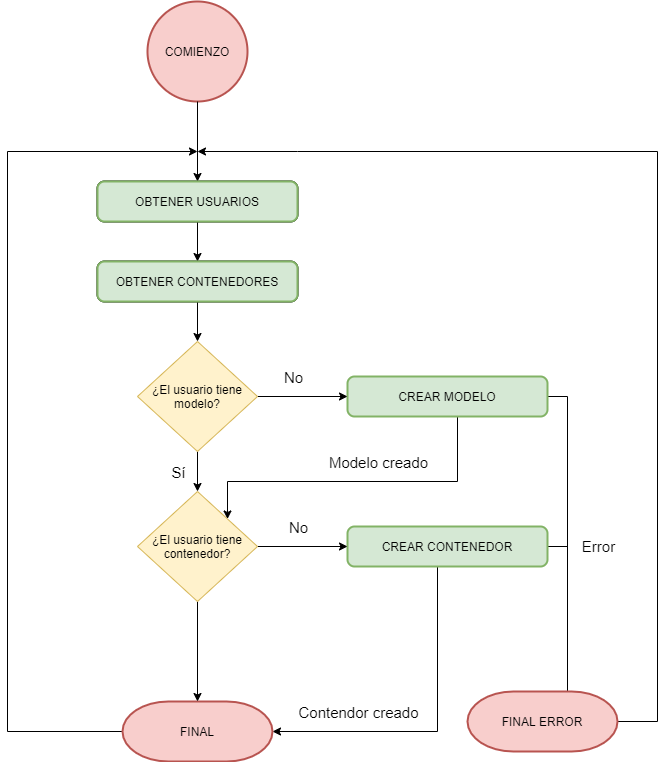
\includegraphics[width=\linewidth,keepaspectratio]{images/orquestation/workflow.png}
        \caption{Flujo del sistema de orquestación}
        \label{fig:orquestation_worflow}
    \end{minipage}
    \begin{minipage}{.49\textwidth}
        \centering
        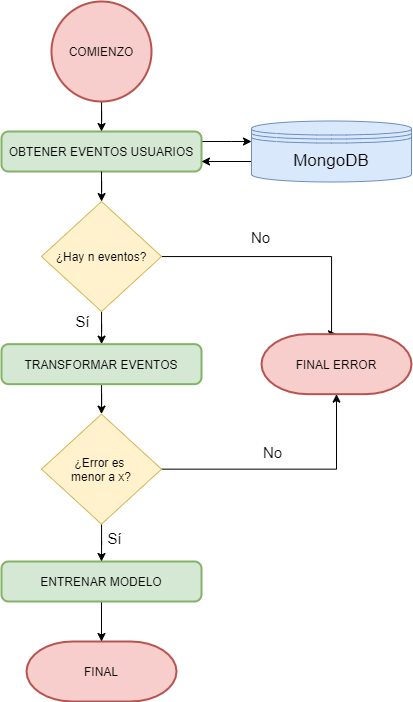
\includegraphics[width=\linewidth,keepaspectratio]{images/orquestation/workflow_model.png}
        \caption{Flujo de creación de modelos}
        \label{fig:workflow_model}
    \end{minipage}

\end{figure}

\subsection{Capa de Datos}

Esta capa se utilizará para almacenar los datos de entrada de manera persistente, para realizar operaciones en el futuro como creación o actualización de nuevos modelos, búsqueda de nuevas características o técnicas de inteligencia artificial.

Como base de datos se ha decidido usar \textit{MongoDB}, una base de datos NoSQL. Los motivos por los que se ha elegido este tipo de base de datos frente a otras (relacional) son:

\begin{itemize}[noitemsep]
    \item \textbf{Velocidad:} Una de las principales ventajas de esta base de datos es la prioridad en manejar lecturas, y en este caso es perfecto para nuestro sistema, debido a que la mayor parte de accesos serán de lectura.
    \item \textbf{Volumen:} La aplicación de captura genera una gran cantidad de datos y por lo tanto, necesitamos una base de datos que funcione en sistemas de \textit{Big Data}.
    \item \textbf{Variabilidad:} La aplicación manejará datos, que pueden no ser consistentes e incluso algunos de ellos pueden modificarse con el tiempo. Este tipo de base de datos no necesitan un esquema para trabajar por lo que las hace ideales para este tipo de casos.
\end{itemize}

\subsubsection{ReplicaSet}

Un \textit{ReplicaSet} en \textit{MongoDB}~[\cref{fig:replica_set}] es un grupo de instancias que mantienen el mismo conjunto de datos. Este sistema permite tener una alta disponibilidad y redundancia de datos.

En el proyecto se crearán tres instancias de \textit{MongoDB} donde la aplicación se conectará a la primaria y las otras instancias se sincronizarán con ella. Una de las ventajas que presenta este sistema es que permite trabajar de manera distribuida, de modo que si un nodo se cae el resto puede asumir el trabajo y el sistema no se ve afectado.

\cfig{images/arquitectura/replicaset.jpg}{Estructura replicaSet~\cite{mongoReplication}}{fig:replica_set}



%\chapter{Metodología}
\label{sec:metodologia}

En esta capítulo se detallará la metodología utilizada para alcanzar los objetivos del proyecto.

\section{Desarrollo incremental}
Este método consiste en una serie de iteraciones, en ventanas de tiempo, en las que al final de las mismas tendremos una parte del producto que el cliente podrá revisar y posteriormente mejorar y/o corregir [\cref{fig:metologia}]

\begin{figure}[htbp!]
    \centering
    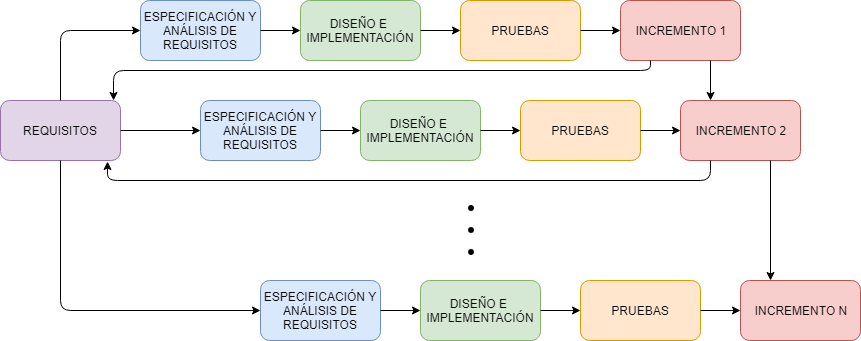
\includegraphics[width=\textwidth, keepaspectratio]{images/arquitectura/metodologia.png}
    \caption{Fases del modelo incremental}
    \label{fig:metologia}
\end{figure}

Esta metodología exige tener dos grupos de usuarios:

\begin{itemize}[noitemsep]
    \item \textbf{Cliente\footnote{Al ser un proyecto de fin de máster, no existe un cliente como tal, por lo que se ha decidido que los directores del proyecto tomen el rol de clientes.}:} Se encarga de revisar el producto al final de las iteraciones.
    \item \textbf{Desarrollador:} Se encarga de desarrollar el producto.
\end{itemize}


Las principales razones por las que se ha elegido esta metodología frente a otras existentes son:

\begin{itemize}[noitemsep]
    \item \textbf{El cliente no sabe exactamente lo que necesita:} Al inicio del proyecto se tenía una idea general del proyecto pero al tratarse de un proyecto con tantas partes diferenciadas los cambios, tecnologías, conexiones~\dots podrían sufrir cambios que implicasen redefinir ciertos conceptos.

    \item \textbf{Obtener un producto usable:} Este proyecto tiene una parte crítica, la de obtener el conjunto de datos lo más rápido posible. Esta parte implica tener una aplicación y el sistema de guardado de información lo antes posible para no bloquear el proyecto.
\end{itemize}

\section{Iteraciones}
El proyecto se dividió en varias iteraciones, en las cuales cada una de ellas proporciona una nueva funcionalidad del sistema.

\subsection{Iteración 0: Búsqueda de información sobre el dominio}
\subsection{Iteración 1: Sistema de captura de información}
\subsection{Iteración 2: Sistema de gestión de colas}
\subsection{Iteración 3: Sistema para el almacenamiento de la información}
\subsection{Iteración 4: Aplicación web de administración}
\subsection{Iteración 5: Comunicación aplicaciones y servidor}
\subsection{Iteración 6: Implementación de la Inteligencia Artificial}
\subsection{Iteración 7: Implementación de máquinas de Inteligencia Artificial}
\subsection{Iteración 8: Automatización del proceso de generación de modelos}


\chapter{Inteligencia Artificial}
\label{sec:ia}

En este capítulo se detallarán los pasos seguidos respecto a la parte de Inteligencia Artificial, el análisis y procesamiento de los datos.


\section{Selección de características}
\label{sec:ia:feature_selection}

Una vez obtenidos los suficientes datos de los usuarios, se han analizado y tratado con el fin de encontrar  posibles valores incorrectos y buscar las mejores características para la predicción.

Cada \textit{input} de un usuario contiene las características relativas a la posición del ratón~[\cref{tab:raw_inputs}]. Los datos son procesados para obtener el conjunto de características más complejas comentadas en la~\cref{tab:transform_inputs} y que se usarán para obtener los modelos finales.


Con las características obtenidas se ha procedido a seleccionar las mejores para intentar optimizar el rendimiento del los algoritmos. Para ello se han utilizado varias técnicas:

\begin{itemize}[noitemsep]
    \item \textbf{Correlación}: Consiste en obtener la relación entre cada característica y eliminar aquellas que poseen un alto nivel~[\cref{fig:correlations_features_selected}]. En nuestro caso se ha tomado \textit{0.8} como el límite máximo de esa relación.
    
    \item \textbf{RFE (Recursive Feature Elimination)}: Esta técnica elimina en cada iteración las características menos importantes, obteniendo en cada una de ellas la predicción~[\cref{fig:rfe}] y el número de características óptimas para nuestro algoritmo. En nuestro caso se han obtenido los valores optimizándolos para las métricas \textit{precision} y \textit{recall}, empleando el algoritmo \textit{Random Forest}, debido a su capacidad de proporcionar un valor de importancia para cada característica.
    
\end{itemize}

\cfig{images/analytics/correlations_features_remove.png}{Matriz de correlación de la selección de características}{fig:correlations_features_selected}

\cfig{images/analytics/rfe.png}{Gráfica de eliminación recursiva de características}{fig:rfe}


Una vez aplicadas las dos técnicas se obtienen los resultados de rendimiento para cada caso, y de esta forma, analizar los resultados obtenidos en función de las métricas de \textit{precision} y \textit{recall}~[\cref{tab:features_remove_result}].

Los resultados muestran valores similares en todas las métricas. Donde más variación existe es en el número de características, y por ello, descartamos la opción de \textit{RFE Recall}, ya que solo tiene en cuenta una característica (\textit{distance}) para obtener la predicción.

De las dos opciones restantes observamos que con más características obtenemos unos mayores valores en ambas métricas, una menor desviación y un tiempo más bajo. Por estas razones se utilizarán las 20 características obtenidas del proceso de correlación.

\begin{table}
    \centering
    \begin{tabularx}{\textwidth}{l C c c c}
        \toprule
        Tipo          & \# características & Precision          & Recall             & Tiempo             \\        \midrule \midrule
        Correlation   & 20                   & 0.914 ($\pm$0.085) & 0.435 ($\pm$0.085) & 3.443 ($\pm$0.090) \\        \midrule
        RFE Precision & 8                    & 0.903 ($\pm$0.109) & 0.432 ($\pm$0.109) & 4.399 ($\pm$0.291) \\        \midrule
        RFE Recall    & 1                    & 0.920 ($\pm$0.074) & 0.450 ($\pm$0.074) & 4.294 ($\pm$0.139) \\
        \bottomrule
    \end{tabularx}
    \caption{\label{tab:features_remove_result}Resultados usando Random Forest}
\end{table}




\subsection{Tratamiento de datos}
\label{sec:ia:data_processing}


El escalado de características a través de la estandarización puede ser un paso muy importante para muchos algoritmos de Inteligencia Artificial. La normalización implica reescalar las características para obtener las propiedades de una distribución normal con una media de cero y una desviación estándar de uno.

Para realizar el escalado se pueden emplear múltiples técnicas como:

\begin{itemize}
    \item \textit{StandardScaler}: Normaliza los datos eliminando la media y escalando los datos de forma que su varianza sea igual a 1.
    \item \textit{RobustScaler}~[\cref{fig:scaler_data}]: Escala los datos de acuerdo al primer y tercer cuartil. 
    \item \textit{PowerTransformer}: Aplica una transformación de potencia a cada característica para que los datos tengan una apariencia Gaussiana, estabilizando la varianza y minimizando la asimetría.
\end{itemize}

En este proyecto se escalaron los datos utilizando la técnica de \textit{RobustScaler}, ya que ofreció mejores resultados para tratar con los valores atípicos (\textit{outliers}).



\cfig{images/analytics/sphx_glr_plot_all_scaling_005.png}{Ejemplo de escalado de datos}{fig:scaler_data}

\section{Selección de algoritmos e hiperparámentros}
\label{sec:ia:rf_selection}

Existen diferentes algoritmos que nos permiten clasificar los datos en diferentes categorías. En este proyecto se realiza una clasificación binaria, es decir, se clasifica basándose en dos etiquetas, si el usuario es legítimo o no legítimo.

\textit{Muli Layer Perceptron}~\cite{rosenblatt1960perceptron}, \textit{Support Vector Machines}~\cite{berwick2003idiot} y \textit{Random Forest}~\cite{Breiman2001} son técnicas que han demostrado un buen rendimiento en este tipo de problemas y es por ello que serán los utilizados para resolver el problema del proyecto.

Para cada uno de los algoritmos seleccionados se procedió a realizar una búsqueda de los hiperparámentros. Estos valores permiten optimizar el ajuste del modelo a los datos con el fin de obtener unos resultados más precisos para el proceso de autenticación.

La cantidad de parámetros y sus valores son distintos en función del algoritmo, por esto se utilizan dos técnicas de búsqueda:

\begin{itemize}
    \item \textbf{Grid Search:} Es una búsqueda exhaustiva de los mejores parámetros de una combinación dada.
    \item \textbf{Random Search:} Es una búsqueda aleatoria sobre una combinación dada.
\end{itemize}


En este proyecto se ha usado la técnica de \textit{Grid Search} como la idónea debido al beneficio/rendimiento sobre ambos procedimientos~\cite{bergstra2012random}.   Para las técnicas de \textit{Multilayer Percetron} y \textit{Random Forest} se configuran una serie de parámetros que modifican su estructura interna. En el \textit{Multilayer Percetron} algunos de estos valores son el número de capas ocultas, número de neuronas por capa y la función de activación. Para \textit{Random Forest} algunos valores son la profundidad máxima del árbol, número de muestras mínimo por hoja  y número mínimo de muestras para crear una nueva hoja. En ambos casos, la modificación de estos parámetros afecta a la creación del algoritmo, decidiendo su estructura interna. Por el contrario, la técnica \textit{SVM} permite la configuración de parámetros que modifican la tolerancia de error. Estos valores son \textit{C}, que controla el margen de error, y \textit{gamma}, que modifica el comportamiento de la función \textit{kernel}. 

La búsqueda de parámetros y posteriores pruebas se han realizado utilizando \textit{Cross Validation}~\cite{kohavi1995study,rao2008dangers} con cinco muestras. Esta técnica tiene un gran impacto a la hora de evitar el \textit{overfitting} debido a una distribución inteligente de los datos.

Como se puede ver en la~\cref{fig:cv_procedure} este procedimiento divide el conjunto inicial de datos en \textit{n} subconjuntos. Esto permite que el entrenamiento que se realiza obtenga resultados más consistentes y reduciendo el \textit{overfitting}, con un coste mayor en tiempo.

\cfig{images/ia/cv_procedure.png}{Funcionamiento de \textit{Cross Validation}}{fig:cv_procedure}

Los parámetros obtenidos como los mejores para el problema a resolver se muestran en la~\cref{tab:best_hyperparams} y sus valores medios para las métricas \textit{recall} y \textit{precision} de cada algoritmo se muestran en la~\cref{tab:compare_clf} y la~\cref{fig:compare_clf}.

Los datos muestran que los tres algoritmos se comportan muy bien a la hora de obtener una predicción, pero debido a la complejidad que podría suponer generar y agrupar tres modelos por usuario, se ha decidido seleccionar \textit{Random Forest} como el algoritmo para el proceso de autenticación final, ya que además de ofrecer un alto rendimiento, también se aprecia una mayor estabilidad a través de la desviación estándar obtenida.


\begin{table}[htbp!]
    \begin{tabular}{c c c c c }
        \toprule
        \multicolumn{5}{c}{\textbf{Multilayer Percetron}                 }                                                    \\ \midrule
        \textit{alpha} & \textit{hidden\_layer\_sizes} & \textit{learning\_rate} & \textit{learning\_rate\_init} & \textit{max\_iter}     \\ \midrule
        0.001                       & (30, 30, 30)                & \textit{adaptive}           & 0.01                 & 1000          \\ \bottomrule \bottomrule

        \multicolumn{5}{c}{\textbf{Support Vector Machines}}                                                                  \\ \midrule
        \multicolumn{2}{c}{\textit{C}}      & \multicolumn{2}{c}{\textit{gamma}}   & \textit{kernel}
        \\ \bottomrule  \bottomrule
        \multicolumn{2}{c}{1000000} & \multicolumn{2}{c}{0.00001} & \textit{rbf}
        \\
        \bottomrule

        \multicolumn{5}{c}{\textbf{Random Forest}}                                                                            \\ \midrule

       \textit{max\_depth} & \textit{max\_features} & \textit{min\_samples\_leaf} & \textit{min\_samples\_split} & \textit{n\_estimators} \\ \midrule

        110                         & 3                           & 5                  & 12                   & 1000          \\ \bottomrule
    \end{tabular}
    \caption{Mejores hiperparámetros para cada algoritmo}
    \label{tab:best_hyperparams}
\end{table}

\begin{table}[htbp!]
    \centering
    \begin{tabular}{c c c }
        \toprule
        Algoritmo            & Métrica   & Media              \\
        \midrule \midrule
        \multirow{2}{*}{RF}  & \textit{precision} & 0.965 ($\pm$0.005) \\
                             & \textit{recall}    & 0.965 ($\pm$0.005) \\ \midrule
        \multirow{2}{*}{MLP} & \textit{precision} & 0.855 ($\pm$0.048) \\
                             & \textit{recall}    & 0.849 ($\pm$0.052) \\ \midrule
        \multirow{2}{*}{SVM} & \textit{precision} & 0.941 ($\pm$0.006) \\
                             & \textit{recall}    & 0.941 ($\pm$0.006) \\
        \bottomrule
    \end{tabular}
    \caption{Media de los resultados de los algoritmos}
    \label{tab:compare_clf}
\end{table}

\cfig{images/analytics/compare_clf.png}{Media de resultados de los algoritmos con su desviación}{fig:compare_clf}




\chapter{Kafka: Sistema de colas}
\label{sec:kafka}

En este capítulo se detallarán las medidas realizadas en \textit{Kafka} para distribuir los datos entre las aplicaciones optimizando la estabilidad del sistema y el tiempo de respuesta.

\section{Envío de datos}

Los datos enviados por el cliente al sistema de colas es el resultado de la combinación de la \textit{metadata}~[\cref{tab:metadata_feature}] y los datos de los eventos~[\cref{tab:raw_inputs}].


\begin{table}[htbp!]
    \centering
    \begin{tabular}{ l  l}
        \toprule
        \textbf{Características} & \textbf{Descripción}                        \\
        \midrule \midrule
        Usuario                  & Nombre del usuario del sistema              \\ \midrule
        Versión aplicación       & Versión de la aplicación                    \\ \midrule
        Sistema Operativo        & Nombre del sistema operativo                \\ \midrule
        Versión del SO           & Versión del sistema operativo               \\ \midrule
        Timestamp                & Fecha del envío de los datos (Formato UNIX) \\
        \bottomrule
    \end{tabular}
    \caption{\label{tab:metadata_feature}Características de la metadata}
\end{table}

Esta definición de los mensajes implica que deben ser producidos y consumidos de manera secuencial. \textit{Kafka} asegura que los mensajes se consumen de manera secuencial solamente cuando existe una partición por cola, esto no permite escalar de forma correcta nuestro sistema, y por lo tanto es necesario definir de nuevo los datos enviados.

\cfig[0.7\linewidth]{images/kafka/acatia-MouseMoveClass.png}{Diagrama de clases de los datos}{fig:mouse_move_class}

La solución obtenida parte por generar bloques de eventos~[\cref{fig:mouse_move_class}] que proporcionan independencia con otros bloques pero que a su cada uno contiene la información necesaria para ser analizada por los modelos. Esta solución también nos proporciona otras mejoras:

\begin{itemize}[noitemsep]
    \item \textbf{Generamos menos tráfico:} La \textit{metadata} solo se envía una vez por grupo.
    \item \textbf{Realizan menos peticiones de red:} Con esta solución se envía una petición por cada bloque.
\end{itemize}

Para decidir el tamaño del bloque se han tenido en cuenta dos limitaciones de nuestro sistema:

\begin{itemize}[noitemsep]
    \item \textbf{\textit{MongoDB}}: El tamaño máximo que se puede guardan en \textit{MongoDB} es de 16~MB
    \item \textbf{\textit{Kafka}}: La configuración por defecto del tamaño de mensaje de \textit{Kafka} es de 1~MB.
\end{itemize}

Con esta información hemos calculado los tamaños de los distintos bloques, de esta manera, saber el número de eventos a enviar por bloque. En la~\cref{tab:events_size} podemos observar los tamaños de evento y de bloque elegidos. La tabla muestra que con 1000 eventos obtenemos un tamaño de bloque inferior a 1~MB, que es el valor límite establecido por defecto en \textit{Kafka}. Además, el tiempo en obtener estos 1000 eventos es de 2 segundos, que determinará el tiempo mínimo necesario para obtener la primera predicción, por lo que es un dato que se debería mantener lo más bajo posible.

Por otra parte, una de las ventajas que se observa al utilizar el bloque como forma de enviar datos entre las aplicaciones, es la reducción del tamaño. Esto implica un consumo de ancho un 72\% menor para el usuario y un 58\% para el servidor.

\begin{table}[htbp!]
    \centering
    \begin{tabular}{ l  c  c  c  c }
        \toprule
        \multirow{2}{*}{\textbf{Datos}} & \multicolumn{2}{c}{\textbf{Evento Único}} & \multicolumn{2}{c}{\textbf{Lista (1000 Eventos)}}                                         \\ \cline{2-5}
                                        & \textbf{Solo}                             & \textbf{Con Metadata}                             & \textbf{Solo} & \textbf{Con Metadata} \\
        \midrule  \midrule
        Evento                          & 44 Bytes                                  & 263 Bytes                                         & 258 KB        & 72 KB                 \\
        \midrule
        Evento Transformado             & 953 Bytes                                 & 1,23 KB                                           & 1239 KBB       & 921 KB                \\
        \bottomrule
    \end{tabular}
    \caption{Tamaño de los eventos enviados uno a uno y agrupados}
    \label{tab:events_size}
\end{table}


\section{Diseño del Escenario}

Una vez definida la estructura de datos dentro del sistema, queda definir las conexiones entre las diferentes aplicaciones. Para ello se plantearon cuatro escenarios distintos, en los cuales se pueden encontrar cuatro procesos:

\begin{itemize}[noitemsep]
    \item \textbf{Splitter}: Es el proceso que divide los datos por usuario.
    \item \textbf{Transform}: Es el encargado de transformar los datos de los eventos del ratón a las características finales.
    \item \textbf{Splitter and Transform}: Es la unión de los dos procesos anteriores, realizando ambos (transformación y división) en una sola máquina.
    \item \textbf{Predictor}: Es el encargado de obtener la predicción para un usuario.
\end{itemize}

\subsection{Escenario 1}

En este escenario [\cref{fig:scene_1}] se plantean tres máquinas, donde la primera máquina (\textbf{Splitter}) recibe los eventos de todos los usuarios y los divide en una cola por usuario, que son enviados primero a la máquina de transformación y después a la de predicción.

\cfig{images/kafka/acatia-escenario_1.png}{Escenario 1}{fig:scene_1}


Este planteamiento presenta una gran desventaja y es la necesidad de tener una máquina de transformación por cada usuario, lo que nos conlleva un alto requisito de recursos.

\subsection{Escenario 2}

Este escenario [\cref{fig:scene_2}] se plantean tres máquinas, pero intercambiando las máquinas de \textbf{Splitter} y \textbf{Transform} con respecto a la versión del escenario anterior.

\cfig{images/kafka/acatia-escenario_2.png}{Escenario 2}{fig:scene_2}


Está versión evita la desventaja del escenario anterior pero añade un problema y es que incrementamos el tamaño de las colas significativamente lo que implica un aumento de los tiempos de envío.

\subsection{Escenario 3}

Este escenario [\cref{fig:scene_4}] cuenta con dos máquinas, delegando el proceso de división a la aplicación de escritorio.
\cfig{images/kafka/acatia-escenario_4.png}{Escenario 3}{fig:scene_4}

Este planteamiento soluciona los problemas de los escenarios anteriores, pero tiene un gran inconveniente y es el almacenamiento de los datos del usuario en la base de datos de \textit{MongoDB}. El proceso de guardado se vuelve más complejo y añade una alta demanda de procesador (uno por usuario) por lo que vuelve un escenario con una escalabilidad baja.

\subsection{Escenario 4}

El último escenario  [\cref{fig:scene_3}] cuenta con dos máquinas, agrupando el \textbf{Splitter} y \textbf{Transform} en una sola.

\cfig{images/kafka/acatia-escenario_3.png}{Escenario 3}{fig:scene_3}

Este escenario soluciona los problemas comentados en el punto anterior, y también los de almacenamiento que teníamos en el escenario anterior ofreciendo un único punto de conexión para almacenar los datos con un coste de 33~ms latencia asumible por el beneficio que aporta.

\chapter{Resultados}
\label{sec:results}

En este capítulo se presentarán los resultados obtenidos aplicando las técnicas mencionadas en los capítulos anteriores.

Primero se analizarán de manera \textit{offline} y acto seguido se analizarán los procesos de creación y predicción de los modelos a lo largo del proceso de \textit{streaming}.


\section{Datos de \textit{Random Forest}}

En la~\cref{tab:rf_results} se pueden observar los resultados obtenidos para diez usuarios con el algoritmo e hiperparámentros seleccionados en la~\cref{sec:ia:rf_selection}. Los datos fueron obtenidos usando la técnica de \textit{CV} con el fin de evitar \textit{overfitting}.

Los resultados muestran la media obtenida para cada usuario sobre las cinco iteraciones del \textit{CV}. En todos los casos se puede observar valores positivos, que superan el 90\% y con una desviación inferior al 1\%.

Estos datos se repiten tanto para la métrica de \textit{precision} como para \textit{recall}, demostrando la fiabilidad del sistema.

\begin{table}[htbp!]
    \centering
    \begin{tabular}{c c c c}
        \toprule
        Usuario & Precision          & Recall             & Time               \\
        \midrule \midrule
        1 &  0.863 ($\pm$0.012) &  0.945 ($\pm$0.012) &  4.943 ($\pm$0.033) \\
        2 &  0.914 ($\pm$0.007) &  0.925 ($\pm$0.007) &  4.914 ($\pm$0.093) \\
        3 &  0.885 ($\pm$0.007) &  0.908 ($\pm$0.007) &  5.091 ($\pm$0.239) \\
        4 &  0.883 ($\pm$0.013) &  0.924 ($\pm$0.013) &  4.907 ($\pm$0.084) \\
        5 &  0.870 ($\pm$0.010) &  0.880 ($\pm$0.010) &  4.919 ($\pm$0.039) \\
        6 &  0.911 ($\pm$0.017) &  0.937 ($\pm$0.017) &  4.882 ($\pm$0.003) \\
        7 &  0.950 ($\pm$0.005) &  0.920 ($\pm$0.005) &  4.898 ($\pm$0.150) \\
        8 &  0.860 ($\pm$0.014) &  0.930 ($\pm$0.014) &  4.904 ($\pm$0.129) \\
        9 &  0.961 ($\pm$0.008) &  0.963 ($\pm$0.008) &  4.929 ($\pm$0.086) \\
        10 &  0.956 ($\pm$0.006) &  0.931 ($\pm$0.006) &  4.860 ($\pm$0.041) \\
        11 &  0.977 ($\pm$0.005) &  0.972 ($\pm$0.005) &  4.789 ($\pm$0.122) \\
        12 &  0.906 ($\pm$0.011) &  0.938 ($\pm$0.011) &  4.920 ($\pm$0.100) \\
        \midrule \midrule
        Media &  0.911 ($\pm$0.010) &  0.931 ($\pm$0.010) &  4.913 ($\pm$0.093) \\
        \bottomrule
    \end{tabular}

    \caption{Resultados de predicción obtenidos}
    \label{tab:rf_results}
\end{table}

Con el fin de comprobar la robustez del sistema se obtuvo el \textit{EER}. En la~\cref{fig:frr_far_user} se puede observar la intersección de las curvas de \textit{FRR} y \textit{FAR} con el fin de obtener de \textit{EER} y cuyos valores se pueden consultar en la~\cref{tab:rf_eer_results}. En ella se puede observar que el ratio es 0.079 con una mínima desviación. Esto implica que el sistema tiene una tasa de fallo inferior al 8\%, lo que ofrece una alta fiabilidad.

\cfig{images/results/frr_far.png}{FAR y FRR de un conjunto de 5 usuarios}{fig:frr_far_user}



\begin{table}[htbp!]
    \centering
    \begin{tabular}{c c}
        \toprule
        Usuario & Equal Error Rate (EER) \\
        \midrule \midrule
        1 &  0.098~($\pm$0.011) \\
        2 &  0.080~($\pm$0.007) \\
        3 &  0.102~($\pm$0.005) \\
        4 &  0.100~($\pm$0.005) \\
        5 &  0.126~($\pm$0.013) \\
        6 &  0.077~($\pm$0.012) \\
        7 &  0.061~($\pm$0.008) \\
        8 &  0.111~($\pm$0.012) \\
        9 &  0.038~($\pm$0.005) \\
        10 &  0.051~($\pm$0.005)\\
        11 &  0.025~($\pm$0.005)\\
        12 &  0.080~($\pm$0.001)\\
        \midrule\midrule
        Media &  0.079~($\pm$ 0.008) \\
        \bottomrule
    \end{tabular}
    \caption{Valores de \textit{EER}}
    \label{tab:rf_eer_results}
\end{table}



\section{Datos de \textit{Streaming}}

Uno de los principales problemas del sistema online es el tiempo que tarda en conseguir los datos necesarios para generar el modelo. En el proyecto se utilizan 20000 eventos, 10000 del usuario legítimo y 10000 de otros usuarios, para crear el modelo. Por lo tanto, necesitamos calcular el tiempo que se tarda en obtener 20000 eventos, debido a que los eventos de múltiples usuarios son generados de manera simultánea. En la~\cref{tab:events_time} se pueden ver los tiempos obtenidos en diez pruebas. En ella se observa la cantidad máxima de eventos generados por un ratón a los diez segundos en diferentes iteraciones. Con estos resultados se ha calculado el tiempo para generar un bloque de 1000 eventos (2.025 segundos) y de 10 bloques.

\begin{table}[htbp!]
    \centering
    \begin{tabular}{c c c c}
        \toprule
        Iteración & Movimientos en 10 segundos & 1 Bloque & 10 Bloques \\
        \midrule\midrule
        1         & 5001.0                     & 1.999    & 19.996     \\
        2         & 4999.0                     & 2.000    & 20.004     \\
        3         & 4994.0                     & 2.002    & 20.024     \\
        4         & 4984.0                     & 2.006    & 20.064     \\
        5         & 4999.0                     & 2.000    & 20.004     \\
        6         & 4993.0                     & 2.002    & 20.028     \\
        7         & 4605.0                     & 2.171    & 21.715     \\
        8         & 4997.0                     & 2.001    & 20.012     \\
        9         & 4983.0                     & 2.006    & 20.068     \\
        10         & 4858.0                     & 2.058    & 20.584     \\
        \midrule\midrule
        Media     & 4941.3                     & 2.025    & 20.250     \\
        \bottomrule
    \end{tabular}
    \caption{Tiempo de obtención los eventos}
    \label{tab:events_time}
\end{table}

Por lo tanto, estos datos nos indican que el tiempo mínimo para que el sistema empiece a realizar predicciones sería de 20.25 segundos.

A estos datos también hay que añadir el tiempo que el sistema tarda en generar el modelo. La~\cref{tab:creation_models_time} muestra el tiempo necesario para obtener los datos de la base de datos, la creación del modelo y la creación de la máquina para realizar predicciones. El tiempo obtenido 29.802 segundos de media. Para todos los modelos, la mayor parte de este tiempo se centra en su creación, en la cual se utiliza solo un núcleo de la máquina. De este modo, podríamos escalar la máquina verticalmente (es decir, incrementando sus recursos) y reducir los tiempos linealmente.


\begin{table}[htbp!]
    \begin{tabularx}{\textwidth}{l |  C C C | c}
        \toprule
        \multirow{2}{*}{Usuarios} & \multicolumn{4}{c}{Tiempos}                                                                 \\ \cline{2-5}
                                                        & Obtener datos & Creación modelo & Creación máquina & Total    \\
        \midrule\midrule
        1    &    4.143 &          21.386 &             1.029 &                26.558 \\
        2    &    5.561 &          20.511 &             1.919 &                27.991 \\
        3    &    5.811 &          22.602 &             1.904 &                30.317 \\
        4    &    5.322 &          24.545 &             0.868 &                30.735 \\
        5    &    4.335 &          20.296 &             1.012 &                25.643 \\
        6    &    4.276 &          23.355 &             1.717 &                29.348 \\
        7    &    4.168 &          21.288 &             1.022 &                26.478 \\
        8    &    5.193 &          25.638 &             1.055 &                31.886 \\
        9    &    4.651 &          24.155 &             1.211 &                30.017 \\
        10    &    4.880 &          20.578 &             1.756 &                27.214 \\
        11    &    4.710 &          24.501 &             1.061 &                30.272 \\
        12    &    4.286 &          25.306 &             1.783 &                31.375 \\
        \midrule\midrule
        Media &    4.778 &          23.168 &             1.856 &                29.802 \\
        \bottomrule
    \end{tabularx}
    \caption{Tiempos de creación de los modelos en el sistema}
    \label{tab:creation_models_time}
\end{table}


Una vez creado el modelo, el sistema empieza a realizar las predicciones de manera inmediata con los datos que se encuentran en las colas. En la~\cref{tab:prediction_time} se muestra el tiempo que tarda un administrador en ver la predicción desde que el bloque se envía al sistema. Como se puede observar, tanto el tiempo de procesado de los eventos como el de predicción son ínfimos en comparación con el tiempo de transporte, que es externo al sistema y depende de factores ajenos como la conexión a internet. Aún con este tiempo, la media se mantiene inferior a los 7 segundos, un tiempo aceptable para ser considerado un sistema de procesamiento en tiempo real en este ámbito de aplicación.

\begin{table}[htbp!]
    \centering
    \begin{tabular}{c | c c c | c}
        \toprule
        \multirow{2}{*}{Usuarios} & \multicolumn{4}{c}{Tiempo}                              \\ \cline{2-5}
                                  & Procesado                  & Predicción & Envío & Total \\
        \midrule\midrule
        1    &      0.4320 & 0.922399 & 8.8620 &           10.216399 \\
        2    &      0.4050 & 0.920659 & 3.3790 &            4.704659 \\
        3    &      0.4470 & 0.923645 & 5.2140 &            6.584645 \\
        4    &      0.3910 & 0.924681 & 4.1190 &            5.434681 \\
        5    &      0.4330 & 0.919187 & 6.5520 &            7.904187 \\
        6    &      0.4216 & 0.921780 & 5.6252 &            6.968580 \\
        7    &      0.4320 & 0.917038 & 8.8620 &           10.211038 \\
        8    &      0.4050 & 0.820295 & 3.3790 &            4.604295 \\
        9    &      0.4470 & 0.820450 & 5.2140 &            6.481450 \\
        10    &      0.3910 & 0.919727 & 4.1190 &            5.429727 \\
        11    &      0.4330 & 0.918583 & 6.5520 &            7.903583 \\
        12    &      0.4216 & 0.920441 & 5.6252 &            6.967241 \\
        \midrule\midrule
        Media &      0.904074 &        0.4320 &         5.6252 &            6.961274 \\


        \bottomrule
    \end{tabular}
    \caption{Tiempos de obtención de predicciones}
    \label{tab:prediction_time}
\end{table}

En la~\cref{fig:acatia_web_auth} se muestra la ventana de administración con los datos obtenidos a lo largo del desarrollo del proyecto. En esta prueba los usuarios utilizaron su ordenador con el sistema de autenticación activado durante su jornada laboral. Los resultados muestran que el sistema de autenticación detecta correctamente a cuatro de los seis usuarios mostrados. Los otros dos usuarios (en color rojo) obtienen un peor porcentaje debido a que durante el transcurso del proyecto cambiaron su ratón por uno ergonómico, demostrando la necesidad de actualizar el modelo utilizado para estos usuarios. Dicho procedimiento se comentará en el~\cref{sec:future_work} como una de las líneas de trabajo futuro.


\cfig{images/results/acatia_web_users.png}{Ventana de administración con datos de autenticación}{fig:acatia_web_auth}


\chapter{Conclusiones}
\label{sec:conclusion}

Los resultados obtenidos del proyecto desarrollado demuestran que es posible un sistema de autenticación, como segundo factor, basado en el comportamiento del usuario y utilizando técnicas de \textit{streaming} para obtener un sistema que es capaz de trabajar en tiempo real a la hora de predecir la legitimidad del usuario.

Para la obtención de datos se creó una aplicación multiplataforma que permitió capturar los eventos generados por el usuario para su posterior análisis. Esta aplicación se instaló en las máquinas de 12 usuarios con el fin de capturar los eventos generados por el ratón.

Con estos datos recopilados se aplicaron diferentes técnicas de Inteligencia Artificial~(\cref{sec:ia}) y los resultados obtenidos después de los diferentes procedimientos obtuvieron un porcentaje de acierto superior al 90\%.

Se implementaron múltiples contenedores con \textit{docker} que nos permitieron automatizar todo el proceso de generación de los modelos de predicción y la obtención de las predicciones. Al usar los contenedores de docker, pudimos aislar los distintos servicios, configurando que solo sean visibles por red entre ellos y que no tengan acceso hacia el exterior, lo que nos ofreció una mayor seguridad a la hora de implantar el sistema en producción.

Para el almacenamiento de los datos se creó un \textit{clúster} de \textit{MongoDB}, lo que nos permitió tener acceso y  redundancia de los datos. Esta configuración final realizada tiene una mayor tolerancia a fallos y facilita el acceso a los datos en caso de fallo en algún nodo.

Para el control y envío de estos datos se implementó una plataforma de gestión de colas (\textit{Kafka}). Esta plataforma envía los datos de los eventos de ratón a la Base de Datos y alimenta el resto de aplicativos con los datos necesarios. Esto nos permite que los procesos de transformación de datos y predicción se realicen con una baja latencia.

Por último, se diseñó y creó una aplicación web que presentase el estado del sistema, mostrando en todo el momento la información relevante sobre los usuarios. Esta presentación permite a un administrador del sistema tener una visión clara del estado actual del sistema.

Como conclusión a título personal, en proyecto se emplearon diferentes tecnologías de diversos ámbitos, lo que me ofreció la posibilidad de investigar sobre dichas tecnologías que a priori no conocía, ampliando de esta manera el conocimiento sobre ciertas áreas como el procesamiento de datos empleando un sistema de colas o la gestión y automatización de una red virtual de ordenadores con docker. 




\chapter{Trabajo Futuro}
\label{sec:future_work}

En este capítulo se comentarán algunos de los posibles desarrollos que se podrían llevar a cabo en un futuro.

\begin{itemize}
    \item \textbf{Refinar el proceso de extracción y selección de características:} Partiendo de la implementación actual, se propone explorar nuevas características en la búsqueda de una optimización de los resultados.
    
    \item \textbf{Actualización de los modelos:} Este tipo de sistemas suelen estar entrenados con un conjunto de datos iniciales que es persistente en el tiempo, pero el comportamiento de una persona puede cambiar con el paso del tiempo, debido a circunstancias como enfermedades o lesiones. Por lo tanto, un aprendizaje que evolucionase con el usuario permitiría obtener una mayor fiabilidad al adaptarse a cambios en los hábitos y comportamiento de los usuarios.    

    \item \textbf{Explorar nuevas técnicas:} Las técnicas elegidas a lo largo del proyecto son una buena base de referencia para el proyecto, pero creemos que diseños basados en tecnologías de \textit{deep-learning} pueden mejorar los resultados obtenidos.
    

    \item \textbf{Combinar técnicas:} Las técnicas usadas se han utilizado de forma independiente, una futura rama de investigación sería combinar las técnicas y obtener de esta formar una predicción por votación.
    
    \item \textbf{Nuevas agrupaciones:} En el proyecto se emplea una agrupación de 1000 eventos con el fin de optimizar el envío y procesamiento de datos. Se plantea realizar un estudio más detallado sobre el tamaño de bloque, buscando de esta forma encontrar un equilibrio entre la mejora de resultados y la degradación en los tiempos de procesamiento.
    
    \item \textbf{Mejorar la web de administración:} La aplicación web permite mostrar la información del estado actual del sistema para realizar las acciones que se consideren oportunas. Este tipo de acciones como un mensaje de aviso o cerrar la sesión del usuario podrían ser implementadas para que se realicen desde la propia aplicación.
\end{itemize}




% --------------------------
% Back matter
% --------------------------
%
{%
    \setstretch{1.1}
    \renewcommand{\bibfont}{\normalfont\small}
    \setlength{\biblabelsep}{0pt}
    \setlength{\bibitemsep}{0.5\baselineskip plus 0.5\baselineskip}
    \printbibliography
    %\printbibliography[nottype=online]
    %\newrefcontext[labelprefix={@}]
    %\printbibliography[heading=subbibliography,title={Webpages},type=online]

}
\cleardoublepage

\listoffigures
\cleardoublepage

\listoftables
\cleardoublepage

%\lstlistoflistings
%\cleardoublepage

%\appendix\cleardoublepage
%\chapter{Apéndice}
\label{sec:appendix}
       % INCLUDE: appendix

\mbox{}

% **************************************************
% End of Document CONTENT
% **************************************************
\end{document}
